\documentclass[journal]{IEEEtran}

\usepackage{cite}
\usepackage{amsmath,amssymb,amsfonts}
\usepackage{graphicx}
\usepackage{textcomp}
\usepackage{xcolor}
\usepackage{booktabs}
\usepackage{multirow}
\usepackage{url}
\usepackage[ruled,vlined]{algorithm2e}
\usepackage{amsthm}
\usepackage{hyperref}

\newtheorem{theorem}{Theorem}
\newtheorem{lemma}[theorem]{Lemma}
\newtheorem{proposition}[theorem]{Proposition}
\newtheorem{corollary}[theorem]{Corollary}
\theoremstyle{definition}
\newtheorem{definition}{Definition}
\theoremstyle{remark}
\newtheorem{remark}{Remark}

\newcommand{\TBD}{\textcolor{red}{\textbf{[TBD]}}}

\def\BibTeX{{\rm B\kern-.05em{\sc i\kern-.025em b}\kern-.08em
    T\kern-.1667em\lower.7ex\hbox{E}\kern-.125emX}}

\begin{document}

\title{FairPoC: Non-IID-Aware Proof of Contribution with Blockchain-Native
Adversarial Defence for Auditable Federated Learning}

\author{\IEEEauthorblockN{Derara Senay Shanka and Peter Shaojui Wang}
\IEEEauthorblockA{Department of Computer Science and Information Engineering\\
National Taiwan University of Science and Technology, Taipei 106, Taiwan\\
Email: derjan06@gmail.com; shaojuiwang@gmail.com}
\thanks{This work extends the conference version presented at IEEE ICBC 2027.
Manuscript received \TBD; revised \TBD; accepted \TBD.}}

\markboth{IEEE Transactions on Information Forensics and Security}%
{Shanka and Wang: FairPoC for Auditable Federated Learning}

\maketitle

%----------------------------------------------------------------------
% [NEW TEXT — fully rewritten from conference abstract]
\begin{abstract}
Open federated learning (FL) marketplaces face two intertwined
threats: unfair reward allocation that discourages high-quality
participation, and rational adversaries who exploit contribution
scoring to inflate their payoffs.
Existing blockchain-FL proposals address at most one of these threats,
and none provides a formally proven economic security guarantee.
This paper presents \textbf{FairPoC}, a unified framework that
resolves both threats through a single on-chain mechanism.
The key insight is that the Proof of Contribution (PoC) score ---
a weighted combination of validation accuracy and median-clipped
gradient norm --- simultaneously serves as a convergence-stable
fairness signal \emph{and} tamper-proof slash evidence in the
\texttt{FairPoC.sol} ERC-20 smart contract.
Clients stake tokens before each round; the contract autonomously
slashes any client whose PoC score falls below $30\%$ of equal
share and redistributes forfeited stakes to honest participants
in the same atomic transaction, with a trust-minimised, on-chain
settlement layer that removes any post-submission reward manipulation
by the aggregator.
% NOTE: the "beyond our conference version" framing and its citation
% were removed on 2026-10-27. The conference paper has not been
% submitted, so it cannot be cited as existing. Restore this framing
% once ICBC accepts; this draft cannot be submitted before then.
We make four contributions:
(i)~a formal Nash equilibrium proof showing that honest
participation is the dominant strategy for any rational client
under stake-and-slash, including a coalition extension;
(ii)~a formal Lemma characterising the self-amplifying failure mode
of max-norm scoring under gradient inflation and proving that
median-clip normalisation eliminates it;
% TODO 2026-10-27: this claims four datasets, but the results tables
% cover only CIFAR-10 and FashionMNIST, and the CIFAR-100 / SVHN data
% on disk does not support a fairness advantage. Either add the tables
% and revise the claim honestly, or narrow this to two datasets.
(iii)~extended experiments on four datasets (CIFAR-10, FashionMNIST,
CIFAR-100, SVHN) with 3 independent seeds and FLTrust, Multi-Krum,
and TMC-Shapley as additional baselines;
(iv)~a formal smart contract security analysis via Slither static
analysis and manual invariant proof.
FairPoC achieves the highest GT-Fairness (a non-circular,
data-quality-grounded metric) across four datasets and four
heterogeneity levels ($\alpha_D \in \{0.1, 0.5, 1.0, 10.0\}$),
with free-rider net-gain $= {-}1.67{\times}$ (economically
irrational to attack) and on-chain deployment requiring no
custom consensus on any EVM-compatible chain.
\end{abstract}

\begin{IEEEkeywords}
federated learning, blockchain, proof of contribution, non-IID,
ERC-20, smart contracts, stake-and-slash, adversarial robustness,
game theory, fairness, gradient norm, information security
\end{IEEEkeywords}

%----------------------------------------------------------------------
\section{Introduction}
\label{sec:intro}

The security of machine learning systems has been studied extensively
from the perspective of data poisoning, model inversion, and
membership inference~\cite{bagdasaryan2020backdoor,bhagoji2019analyzing}.
Yet a largely overlooked attack surface in federated learning (FL) is
the \emph{reward mechanism} itself.
As FL moves from academic settings into open cross-organisational
marketplaces --- where mutually distrusting participants contribute
data and compute in exchange for token rewards --- rational adversaries
emerge who have no interest in degrading model accuracy but are
strongly incentivised to maximise their reward share at the expense of
honest contributors~\cite{lin2019free, song2019profit}.
These economic attackers are qualitatively different from the
data-poisoning adversaries studied in prior
work~\cite{bhagoji2019analyzing}: they need not corrupt the model to
profit, and standard Byzantine-robust aggregation rules that filter
divergent gradients provide no deterrence against a free-rider who
submits the current global model unchanged.

The root vulnerability is structural.
Existing FL incentive schemes compute contribution scores at a central
aggregator and distribute rewards through the same trusted
server~\cite{wang2020measure, gradient_driven_fairness2021}.
An aggregator that is compromised, colluding, or simply
self-interested can silently reassign rewards with no publicly
verifiable record.
Blockchain smart contracts offer a well-known remedy for tamper-evident
enforcement~\cite{buterin2014ethereum}, and several blockchain-FL
proposals have emerged~\cite{kim2019blockchained, bladefl2022,
poshapley2023, behera2021federated}.
However, none of these works close the economic attack surface:
they either defer adversarial defence to off-chain filtering (where it
remains under the control of the aggregator), use contribution metrics
that collapse at convergence (peer-voting and Shapley-based signals
become uninformative once accuracy saturates), or require custom
consensus protocols that limit real-world deployability.
Existing on-chain stake-and-slash systems for FL (e.g.\
FLock~\cite{dong2022flock}) are engineering artifacts: they
demonstrate economic deterrence empirically but do not prove it.
Critically, no existing work \emph{formally proves} that a
specific contribution score coupled to a smart contract creates a
Nash equilibrium in which honest participation is the dominant
strategy for any rational client.

A second challenge compounds the first: under non-IID data
distributions --- the norm in real deployments where each client holds
a skewed, domain-specific data slice --- standard contribution metrics
based on Shapley values or leave-one-out (LOO) accuracy
\emph{collapse to zero} as the global model
converges~\cite{poshapley2023}.
This means that by late training, every client looks equally
valuable regardless of actual data quality, making contribution-based
rewards indistinguishable from uniform allocation.
The adversarial consequence is serious: a free-rider who submits zero
updates scores similarly to an honest contributor once the global
model saturates, defeating score-based slashing unless the scoring
signal remains informative throughout training.

We address both challenges simultaneously with \textbf{FairPoC}.
The central design insight is that normalised gradient norm ---
unlike Shapley or LOO margins --- is an intrinsic property of each
client's local data distribution that \emph{does not depend on other
clients' contributions} and therefore remains non-degenerate throughout
training.
We encode a PoC score combining gradient norm and validation accuracy
directly in an ERC-20 smart contract, where the same score that
determines each client's reward also serves as tamper-proof,
immutable evidence for autonomous slashing.
A client that scores below $30\%$ of equal share is slashed and
permanently blacklisted in the same atomic transaction that distributes
rewards, with no trusted intermediary able to intervene.

This paper makes the following contributions:
\begin{enumerate}
  \item \textbf{Convergence-stable PoC score.}
        A non-IID-aware score combining validation accuracy with
        median-clipped gradient norm that remains informative and
        client-differentiated throughout all training rounds,
        directly addressing the convergence instability of
        Shapley- and LOO-based methods.

  \item \textbf{Blockchain-native adversarial defence.}
        A stake-and-slash mechanism encoded \emph{atomically} in
        \texttt{FairPoC.sol}: the PoC score simultaneously
        determines reward and provides tamper-proof slash evidence,
        eliminating the need for any trusted intermediary in the
        exclusion decision.

  \item \textbf{Formal game-theoretic security guarantee.}
        Theorem~\ref{thm:nash} proves that honest participation is
        the dominant strategy under stake-and-slash for any rational
        single attacker; the appendix extends this to a coalition
        of up to $\lfloor n/3 \rfloor$ colluding clients.

  \item \textbf{GradScale amplification lemma.}
        Lemma~\ref{lem:amplification} formally characterises a
        self-amplifying failure mode in max-norm contribution
        scoring under gradient inflation, and
        Corollary~\ref{cor:mc_fix} proves that median-clip
        normalisation eliminates it.

  \item \textbf{Comprehensive empirical validation.}
        Evaluation on 4 datasets (CIFAR-10, FashionMNIST, CIFAR-100,
        SVHN), 4 heterogeneity levels
        ($\alpha_D \in \{0.1, 0.5, 1.0, 10.0\}$),
        3 independent seeds, and 6 baselines including TMC-Shapley,
        FLTrust, and Multi-Krum, plus three adversarial attack types
        using a non-circular GT-Fairness metric.
\end{enumerate}

% ==================================================================
% EXTENSION STATEMENT, DISABLED 2026-10-27.
% Two problems, both of which must be fixed before this is restored:
%  (1) It cites a conference paper that does not exist yet.
%  (2) It lists the CIFAR-100 and SVHN experiments as a contribution.
%      Those runs completed after the tables were written and do NOT
%      support the claim: FairPoC ties FedAvg on accuracy and loses on
%      GT-Fairness in 7 of 8 cells. Listing them as an extension while
%      the conclusion claims 6-of-8 superiority is worse than omitting
%      them. Decide what to do with those results first.
% ==================================================================
%This paper substantially extends our conference
%version~\cite{fairpoc_icbc2027}.
%The new contributions are: the formal game-theoretic proof
%(Section~\ref{sec:gametheory}), the GradScale amplification lemma
%(Section~\ref{subsec:amplification}), the contract formal
%verification (Section~\ref{sec:contract_verification}), extended
%experiments on 2 additional datasets (CIFAR-100, SVHN) with
%3 independent seeds
%(Section~\ref{sec:experiments}), and the coalition attack analysis
%(Appendix~\ref{appendix:coalition}).
%All text has been substantially rewritten; shared experimental
%results are presented with multi-seed statistics not included
%in the conference version.

%----------------------------------------------------------------------
\section{Related Work}
\label{sec:related}

\subsection{Contribution Measurement in FL}

Measuring each client's marginal contribution to a collaborative
model is a well-studied problem rooted in cooperative game
theory~\cite{shapley1953value}.
The Shapley value assigns each client a reward equal to its average
marginal contribution across all possible client orderings, and has
been advocated as the principled fairness criterion for FL
incentive design~\cite{song2019profit, wang2020measure}.
However, exact Shapley computation requires $O(2^n)$ model
evaluations, making it impractical beyond toy settings.
Ghorbani and Zou~\cite{ghorbani2019data} propose Truncated Monte
Carlo (TMC) Shapley, reducing complexity to $O(T \cdot n)$ with $T$
random permutations per round.
Even so, both exact and approximate Shapley values share a deeper
problem: as FL training converges and the global model saturates,
marginal contributions collapse toward zero --- by late rounds,
removing any single client causes negligible accuracy loss,
making all clients appear equally
valuable~\cite{poshapley2023}.
This convergence instability means Shapley-based rewards
lose discriminative power precisely when sustained participation
incentives matter most.

Leave-one-out (LOO) methods suffer from the same instability.
Recent work proposes gradient-based alternatives: Xu
et al.~\cite{gradient_driven_fairness2021} reward each client
proportionally to the inner product of its gradient with the
consensus gradient direction.
Inner-product scoring is convergence-stable in principle, but is
sensitive to gradient alignment and degrades in non-IID settings
where client gradients diverge in direction.
FairPoC instead uses gradient \emph{norm} --- a scalar signal
that captures the scale of a client's local update independently
of direction --- which remains non-degenerate throughout training
and is robust to non-IID divergence.
Unlike all the above approaches, FairPoC encodes the scoring
outcome in an ERC-20 smart contract, eliminating the trusted
central coordinator required for reward distribution.

\subsection{Incentive Mechanisms and Fairness in FL}

Beyond contribution scoring, the incentive design problem in FL
encompasses mechanism design, reputation, and fairness notions
from both economics and computer science.

\textbf{Auction and contract theory.}
Zhan et al.~\cite{zhan2021incentive} frame FL client recruitment
as a reverse auction: clients submit bids specifying their
requested payment for contributing data, and the server selects
a cost-minimising subset satisfying a quality constraint.
Ding et al.~\cite{ding2020optimal} apply contract theory to FL
with multi-dimensional private information (data quality and
quantity), designing a menu of contracts that induces truthful
reporting under incentive-compatibility constraints.
These mechanisms are theoretically principled but assume a
trustworthy server to evaluate bids and enforce payments ---
an assumption FairPoC removes by encoding enforcement on-chain.

\textbf{Reputation systems.}
Kang et al.~\cite{kang2019incentive} combine reputation scores
with contract theory to selectively recruit high-quality workers
in a mobile crowdsensing FL setting.
Reputation is maintained by the server and updated based on
historical contribution quality.
FairPoC's stake-and-slash mechanism provides a complementary
guarantee: rather than discouraging low-quality clients through
reduced future recruitment, it imposes an immediate economic
penalty enforced immutably on-chain, providing a stronger
deterrence that does not rely on the server's honesty in
maintaining reputation records.

\textbf{Fairness notions.}
Multiple fairness criteria have been proposed for FL:
proportional fairness (reward $\propto$ contribution),
Pareto-optimality, and equitability~\cite{song2019profit}.
FairPoC adopts a \emph{non-circular} ground-truth fairness metric
(GT-Fairness, Section~\ref{sec:experiments}) that derives the
reference allocation from the data partition itself, independent
of any scoring method, avoiding the self-referential circularity
that affects metrics grounded in the scores being evaluated.

\subsection{Blockchain-Assisted FL}

The idea of combining blockchain with FL for auditability was
introduced by Kim et al.~\cite{kim2019blockchained}, who propose
recording model updates on a permissioned blockchain to create
an immutable training log.
BLADE-FL~\cite{bladefl2022} goes further, replacing the central
aggregator with a blockchain-based consensus protocol where
clients compete to generate blocks containing verified model
updates, achieving Byzantine resilience through block validation.
PoCL~\cite{pocl2024} proposes a multi-winner consensus algorithm
that repurposes proof-of-work computation for FL training,
coupling model improvement to block mining incentives.
PoShapley-BCFL~\cite{poshapley2023} encodes Shapley-based
contribution scores into a custom blockchain consensus, explicitly
linking training contribution to block rewards.
Behera et al.~\cite{behera2021federated} deploy Ethereum smart
contracts with a scalar contribution metric derived from weight
update magnitude, demonstrating the viability of ERC-20-based
reward distribution for FL.

DeepChain~\cite{weng2021deepchain} provides privacy-preserving
auditable FL via on-chain gradient commitments, demonstrating
that blockchain can enforce training integrity; however, it does
not address contribution fairness or economic deterrence against
free-riders.
CFFL~\cite{lyu2020cffl} formulates collaborative fairness as a
multi-player game and shows that higher-contributing clients should
receive higher-accuracy models; the enforcement mechanism is
centralised, leaving it susceptible to aggregator manipulation.
RFFL~\cite{xu2020rffl} extends collaborative fairness with
reputation-weighted aggregation.
PoCQ~\cite{pocq2023} introduces a proof-of-quality concept for
FL incentives but relies on a centralised quality oracle and does
not provide economic deterrence via on-chain staking.
The closest prior work to FairPoC is FLock~\cite{dong2022flock,dong2024flock},
a blockchain-based FL system that uses Ethereum smart contracts with an
on-chain stake-and-slash mechanism to penalise malicious clients, combined
with a P2P model-evaluation voting protocol.
FLock demonstrates that on-chain economic deterrence for FL is feasible,
and FairPoC builds on this direction.
However, FLock's contribution signal relies on peer voting, which
collapses to uniform scores as the global model converges (all
models look equally good to evaluators once accuracy saturates).
FLock does not characterise this failure mode, does not provide an
alternative signal that remains informative post-convergence, and
does not offer a formal game-theoretic proof that honest participation
is the dominant strategy under its mechanism.
None of the systems above combines all three properties: a
contribution signal that remains valid at convergence under non-IID
data, on-chain enforcement without custom consensus, and a formal
Nash equilibrium guarantee.

\begin{table}[t]
\centering
\caption{Positioning of FairPoC against closest related works.
  \checkmark = property satisfied; $\times$ = not satisfied;
  $\approx$ = partially or under restrictive conditions.}
\label{tab:positioning}
\small
\begin{tabular}{lccc}
\toprule
System & Convergence-stable score & On-chain enforcement & Formal NE proof \\
\midrule
FLock~\cite{dong2022flock}            & \texttimes & \checkmark & \texttimes \\
PoShapley-BCFL~\cite{poshapley2023}   & \texttimes & $\approx$  & \texttimes \\
Xu et al.~\cite{gradient_driven_fairness2021} & \checkmark & \texttimes & \texttimes \\
Behera et al.~\cite{behera2021federated}      & \texttimes & \checkmark & \texttimes \\
\textbf{FairPoC (ours)}               & \checkmark & \checkmark & \checkmark \\
\bottomrule
\end{tabular}
\end{table}

FairPoC occupies the intersection of these three threads (Table~\ref{tab:positioning}).
We use standard ERC-20 token interfaces rather than custom
consensus protocols, enabling deployment on any EVM-compatible chain.
We replace peer-voting and Shapley-based signals with median-clipped
gradient norm, which remains client-differentiated throughout training
where peer-voting and Shapley methods lose discriminative power.
Most importantly for TIFS readers, we provide a formal game-theoretic
proof that the combined scoring-and-slashing mechanism makes honest
participation the dominant strategy --- a guarantee absent from all
prior blockchain-FL incentive works.

\subsection{Adversarial Attacks and Defences in FL}

\textbf{Model and gradient poisoning.}
Bhagoji et al.~\cite{bhagoji2019analyzing} demonstrate that a
single Byzantine client can substantially degrade global model
accuracy by scaling its update to dominate aggregation.
Bagdasaryan et al.~\cite{bagdasaryan2020backdoor} show that a
constrained adversary can inject a persistent backdoor into the
global model while maintaining benign-looking updates, evading
anomaly-based detection.
These attacks target model \emph{accuracy}; FairPoC addresses
a complementary class of attacks that target the \emph{reward
mechanism} without necessarily harming accuracy.

\textbf{Free-rider attacks.}
Lin et al.~\cite{lin2019free} formally define the free-rider
problem in FL: a selfish client submits the current global model
as its local update (zero gradient), contributing nothing while
collecting a proportional reward.
They show that standard Byzantine-robust aggregators (Krum,
Trimmed Mean) do not detect free-riders because zero updates
are not statistically divergent from convergent honest updates.
FairPoC detects free-riders through near-zero gradient norm,
which falls below the slash threshold regardless of validation
accuracy, and enforces exclusion on-chain.

\textbf{Byzantine-robust aggregation.}
A rich line of work proposes robust aggregation rules that
tolerate up to $f < n/2$ Byzantine
clients~\cite{blanchard2017machine, yin2018byzantine}.
Krum selects the update closest to its $n-f-2$ nearest neighbours;
Trimmed Mean discards the extreme $\beta$ fraction before averaging;
FLTrust normalises each update by a trusted server-side reference
gradient.
These methods are orthogonal to FairPoC's stake-and-slash
mechanism and can be composed with it: FairPoC provides economic
deterrence while robust aggregation provides structural protection.
Crucially, all existing robust aggregation rules are enforced by
the aggregator and can be circumvented if the aggregator is
compromised --- stake-and-slash is the first mechanism to enforce
exclusion immutably on-chain.

\textbf{Economic deterrence.}
On-chain economic penalties for FL misbehaviour have been explored in
prior work --- most notably FLock~\cite{dong2022flock,dong2024flock},
which applies stake-and-slash via Ethereum smart contracts to deter
model poisoning.
FairPoC shares this direction but makes two contributions that
distinguish it: (i)~the slashing signal is a convergence-stable,
non-IID-aware gradient-norm score rather than peer-voting (which
collapses at convergence), and (ii)~we formally prove that the
combined scoring-and-slashing mechanism constitutes a Nash equilibrium
in which honest participation is the \emph{dominant} strategy for any
rational client, including coalition attackers.
No prior blockchain-FL system provides this formal guarantee.

%----------------------------------------------------------------------
\section{System Design}
\label{sec:design}

\subsection{Architecture Overview and Trust Assumptions}

FairPoC involves three roles: \emph{clients}, a semi-trusted
\emph{aggregator}, and an \emph{immutable smart contract} deployed
on an EVM-compatible blockchain.
Clients hold private training data and submit model updates each
round.
The aggregator collects updates, computes PoC scores, and submits
them on-chain; it is the single point of contact with the contract
but \emph{cannot influence the outcome}: reward and slash decisions
are computed deterministically by the contract code from the
submitted scores and enforced atomically, so a dishonest or
compromised aggregator cannot over-pay, under-slash, or retroactively
alter any distribution.
The blockchain provides global, tamper-resistant state: every round's
scores, reward transfers, and slash events are permanently logged
and auditable by any participant.

This trust model is weaker than systems requiring an honest-majority
aggregator (e.g., blockchain-based gradient commitments~\cite{weng2021deepchain})
and stronger than purely off-chain defences (e.g., BLADE-FL~\cite{bladefl2022})
that rely on the aggregator to correctly apply the filter.
The economic stakes in \texttt{FairPoC.sol} make rational deviations
unprofitable without any assumption on the aggregator's honesty.

Algorithm~\ref{alg:fairpoc} shows the full per-round protocol
including staking, contribution scoring, slashing, and reward
distribution.

\begin{algorithm}[t]
\caption{FairPoC Training Protocol (full stake-and-slash flow)}
\label{alg:fairpoc}
\SetKwInOut{Input}{Input}
\SetKwInOut{Output}{Output}
\Input{Global model $\theta^{(0)}$, rounds $T$, clients $\mathcal{C}=\{1\ldots n\}$,
       stake amount $\delta$, reward pool $R$, slash threshold $\tau_s$}
\Output{Trained model $\theta^{(T)}$; token ledger for each client}
\BlankLine
\For{$t = 1$ \KwTo $T$}{
  \tcp{Phase 1 — Staking (on-chain)}
  \ForEach{$i \in \mathcal{C} \setminus \texttt{blacklist}$}{
    Client $i$ calls \texttt{stake(t)}: transfers $\delta$ tokens to contract\;
  }
  \BlankLine
  \tcp{Phase 2 — Local Training (off-chain)}
  Aggregator broadcasts $\theta^{(t-1)}$ to active clients\;
  \ForEach{active client $i$}{
    Minimise $\mathcal{L}_i(\theta)$ for $E$ local epochs $\Rightarrow \Delta w_i = \theta_i^{(t)} - \theta^{(t-1)}$\;
  }
  Clients transmit $\{\Delta w_i\}$ to aggregator\;
  \BlankLine
  \tcp{Phase 3 — PoC Scoring (off-chain, aggregator)}
  \ForEach{active client $i$}{
    Compute $s_i = \alpha_p \cdot \mathrm{ValAcc}_i + \beta_p \cdot \mathrm{GradNorm}_i$ (Eq.~\ref{eq:poc})\;
  }
  Normalise: $\hat{s}_i \leftarrow s_i / \sum_j s_j$\;
  \BlankLine
  \tcp{Phase 4 — On-chain Settlement (atomic)}
  Aggregator calls \texttt{submitAndSettle}($\mathbf{s}$, $\tau_s$, $R$, $t$)\;
  \ForEach{client $i$}{
    \uIf{$\hat{s}_i < \tau_s / n$}{
      Add $i$ to \texttt{blacklist}; transfer $\delta$ to slash pool $P_{\mathrm{slash}}$\;
    }
  }
  $\mathcal{H}_t \leftarrow \{i : i \notin \texttt{blacklist}\}$\tcp*{honest set this round}
  \ForEach{$i \in \mathcal{H}_t$}{
    $r_i \leftarrow \dfrac{s_i}{\sum_{j\in\mathcal{H}_t} s_j}\cdot(R + P_{\mathrm{slash}})$;
    transfer $r_i$ from contract to client $i$\;
  }
  \BlankLine
  \tcp{Phase 5 — Aggregation (off-chain)}
  $\theta^{(t)} \leftarrow \displaystyle\sum_{i \in \mathcal{H}_t}
    \frac{s_i}{\sum_{j \in \mathcal{H}_t} s_j}\,\theta_i^{(t)}$\;
}
\end{algorithm}

\subsection{Smart Contract Architecture}
\label{subsec:contract_arch}

\texttt{FairPoC.sol} is a fixed-supply ERC-20 token contract
(1{,}000{,}000 tokens at deployment) augmented with three
FL-specific functions.
ERC-20 was chosen deliberately: it provides a well-audited token
interface compatible with any EVM wallet and exchange, enabling token
liquidity without custom infrastructure.
The three additional functions and their security invariants are:

\textbf{\texttt{stake(uint256 round)}.}
Each active client deposits $\delta$ tokens before round $t$ begins.
The function reverts if called for a past or already-settled round,
preventing replay and double-staking.
Deposited tokens are held in the contract's internal balance and
cannot be withdrawn by any party, including the aggregator, until
\texttt{submitAndSettle} executes.

\textbf{\texttt{submitAndSettle(address[] clients, uint256[] scoresE4, uint256 thresholdE4, uint256 round)}.}
The aggregator submits the PoC score vector as 4-decimal fixed-point
integers ($s_i \times 10^4$) to avoid floating-point in Solidity.
The function iterates once over the client list in deterministic
order, computing the normalised share $\hat{s}_i$ entirely on-chain
and slashing any client whose share falls below
$\tau_s \cdot \frac{1}{n}$ ($\tau_s = 0.30$).
Reward distribution follows in the same transaction: the slashed
pool plus the round pool $R$ are divided proportionally among
unslashed clients, with each transfer emitting an ERC-20
\texttt{Transfer} event for public audit.
The $n^2$ gas cost of the pairwise contribution comparison is avoided
entirely: the slash test requires only one comparison per client
($O(n)$ total).

\textbf{\texttt{isBlacklisted(address client)}.}
A public view function returning whether a client has been
permanently excluded. Clients can query this before staking to
avoid wasting gas on a round in which they are blacklisted.

The two-function decomposition (\texttt{\_classifyAndSlash} and
\texttt{\_distribute}, implemented as \texttt{internal} helpers to
stay within the EVM's 16-variable stack limit) is the key structural
change from the conference version.
It enables Slither static analysis without stack-depth errors and
makes the slash logic independently verifiable
(Section~\ref{sec:contract_verification}).

\subsection{Aggregator Interface and Off-Chain Communication}

The aggregator maintains a secure channel with each client for
receiving model updates.
It does not require access to clients' private datasets or gradients
beyond what is submitted each round.
All decisions that affect token balances are made on-chain;
the aggregator's off-chain scoring is input-only.
A compromised aggregator that submits false scores would still be
subject to the on-chain threshold: it cannot grant reward to a
zero-gradient client (whose $\mathrm{GradNorm} = 0$) without that
client's raw score falling below the slash threshold, triggering
automatic slashing.

%----------------------------------------------------------------------
\section{Non-IID-Aware Proof of Contribution}
\label{sec:poc}

\subsection{Motivation: Why Existing Scoring Signals Fail Under Non-IID}
\label{subsec:poc_motivation}

Before defining the PoC score, we explain why the two most common
alternatives are insufficient for non-IID FL.

\textbf{Cosine similarity (BLADE-FL~\cite{bladefl2022}).}
Cosine similarity measures angular alignment between a client's
update and the average update direction.
Under non-IID partitioning, clients holding rare classes produce
updates that \emph{diverge} from the mean, because their local loss
surface is oriented differently from the majority.
A cosine-similarity filter therefore systematically penalises
clients with rare data --- the very clients whose contributions are
most valuable for generalisation.
This is not a deficiency of BLADE-FL's Byzantine-detection goal;
it is a structural incompatibility between the cosine metric and
the incentive goal.

\textbf{Leave-one-out / Shapley values.}
LOO contribution $\delta_i^t = \mathrm{Acc}(\theta^t) -
\mathrm{Acc}(\theta_{-i}^t)$ measures how much the global accuracy
drops when client $i$ is removed.
Early in training this signal is informative; however, as the model
converges, marginal accuracy improvements from any single client
approach zero (Fig.~\ref{fig:stability}).
By round 30 of 50, the LOO signal collapses to near-zero for all
clients simultaneously, making it impossible to distinguish high-
from low-quality contributors.
TMC-Shapley~\cite{ghorbani2019data} inherits this limitation
(Section~\ref{subsec:shapley}) and incurs $O(nT)$ forward passes
per round.

Both limitations motivate a contribution signal that is (i) scale-
sensitive rather than direction-sensitive, (ii) non-degenerate at
convergence, and (iii) computable in $O(n)$ per round.

\subsection{PoC Score Definition}
\label{subsec:poc_def}

We decompose each client's contribution into two orthogonal
dimensions: model quality and data diversity.
Model quality is measured directly by validation accuracy on a
shared server-side validation set; data diversity by the scale
of the parameter update, which encodes how far the client's
local data distribution pushes the model from its current state.

\begin{equation}
  s_i = \alpha_{\mathrm{p}} \cdot \mathrm{ValAcc}_i
        + \beta_{\mathrm{p}} \cdot \mathrm{GradNorm}_i
  \label{eq:poc}
\end{equation}
with $\alpha_{\mathrm{p}} = 0.7$ and $\beta_{\mathrm{p}} = 0.3$
(selected by ablation; Section~\ref{subsec:ablation_beta}).
$\mathrm{ValAcc}_i \in [0,1]$ is the top-1 accuracy of client $i$'s
local model on the shared validation set, evaluated after local
training but before aggregation.
$\mathrm{GradNorm}_i \in [0,1]$ is the normalised gradient norm
defined in Section~\ref{subsec:gradnorm}.

The coefficients $\alpha_p$ and $\beta_p$ sum to $1.0$ by convention,
but normalisation is not required for correctness: dividing each
$s_i$ by $\sum_j s_j$ for aggregation is equivalent to any positive
scaling of the coefficients.
The choice $\alpha_p > \beta_p$ reflects the empirical observation
that validation accuracy is a lower-variance signal than gradient
norm across all tested datasets and heterogeneity levels; the
gradient norm component provides the non-IID diversity correction.

\subsection{Gradient Norm as a Non-IID Diversity Signal}
\label{subsec:gradnorm}

The raw parameter update $\Delta w_i = \theta_i^{(t)} - \theta^{(t-1)}$
reflects the displacement induced by client $i$'s local data.
A client holding data from a narrow class slice produces a large
update because its local loss surface is far from the global optimum;
a client that closely mirrors the global distribution produces a
smaller, lower-informational update.
Under Dirichlet non-IID partitioning, the correlation between
$\|\Delta w_i\|_2$ and the data-quality ground truth
$\mathrm{gt}_i$ (Section~\ref{subsec:gt_fairness}) is
empirically $r \geq 0.72$ across all tested configurations,
confirming that gradient magnitude is a reliable proxy for
distributional contribution.

Two normalisation variants handle the adversarial case:
\begin{align}
  \mathrm{GradNorm}_i^{\mathrm{max}}
    &= \frac{\|\Delta w_i\|_2}{\max_j \|\Delta w_j\|_2}
  \label{eq:gradnorm_max} \\
  \mathrm{GradNorm}_i^{\mathrm{mc}}
    &= \frac{\min\!\left(\|\Delta w_i\|_2,\;
       \bar{g}\right)}{\bar{g}},\quad
       \bar{g} \triangleq \mathrm{med}_j\|\Delta w_j\|_2
  \label{eq:gradnorm_mc}
\end{align}
Max-norm normalisation (Eq.~\ref{eq:gradnorm_max}) is used in clean
settings; median-clip (FairPoC-MC, Eq.~\ref{eq:gradnorm_mc}) is the
default in all adversarial experiments.
The median is computed over the full client set each round, requiring
$O(n)$ comparisons with no server-side model forward pass.

\textbf{Why the median specifically?}
The median is the breakdown-point-optimal estimator for shift
contamination: a minority of $\lfloor(n-1)/2\rfloor$ adversarial
clients cannot move the median beyond the honest client range.
The mean would be dominated by any single client scaling its update
by $S \gg 1$; the median is unaffected provided fewer than half the
clients inflate.
For $n = 10$ clients and one attacker (our experimental setting),
the median is determined by the 5th and 6th ordered norms, both of
which belong to honest clients.

\textbf{Convergence stability.}
Unlike LOO and Shapley, the gradient norm is an \emph{intrinsic}
property of a client's data distribution and does not depend on the
marginal contribution to global accuracy.
Even at convergence, clients with different data distributions
continue to produce distinguishably scaled updates: the ordering
$\|\Delta w_i\| > \|\Delta w_j\|$ when client $i$ holds rarer
classes is preserved throughout training.
Fig.~\ref{fig:stability} confirms this empirically: per-client
gradient norms remain client-ordered and bounded away from zero
for all 50 rounds, while LOO margins collapse after round 30.

\subsection{GradScale Self-Amplification and the Median-Clip Fix}
\label{subsec:amplification}

\begin{lemma}[GradScale Self-Amplification]
\label{lem:amplification}
Let one client $a$ scale its update by factor $S \gg 1$ while $n-1$
honest clients submit unmodified updates.
Under max-norm scoring (Eq.~\ref{eq:gradnorm_max}):
\begin{equation}
  \mathrm{GradNorm}_a^{\mathrm{max}} = 1.0, \quad
  \mathrm{GradNorm}_i^{\mathrm{max}} \leq \frac{1}{S}
  \quad \forall i \neq a.
  \label{eq:amplification}
\end{equation}
The attacker's aggregation weight satisfies:
\begin{equation}
  w_a \geq \frac{\alpha_p \cdot \mathrm{ValAcc}_a + \beta_p}
               {\alpha_p \cdot \bar{V} + \beta_p/S}
  \xrightarrow{S \to \infty} \frac{1}{\alpha_p \bar{V}}
  \label{eq:weight_amplification}
\end{equation}
where $\bar{V}$ is the mean validation accuracy.
For $\bar{V} < 1$, this exceeds $1/n$, giving the attacker
super-proportional aggregation weight.
\end{lemma}

\begin{proof}
Under GradScale by factor $S$, $\|\Delta w_a\|_2 = S \|\Delta w_a^0\|_2$
where $\Delta w_a^0$ is the unattacked update.
Since $S \gg 1$, client $a$ becomes the maximum, so
$\mathrm{GradNorm}_a^{\mathrm{max}} = 1.0$.
For any honest client $i$: $\|\Delta w_i\|_2 \leq \|\Delta w_a^0\|_2$
under typical gradient magnitudes, so
$\mathrm{GradNorm}_i^{\mathrm{max}} = \|\Delta w_i\|_2 / \|\Delta w_a\|_2
\leq \|\Delta w_a^0\|_2 / (S\|\Delta w_a^0\|_2) = 1/S$.
The score $s_a = \alpha_p \mathrm{ValAcc}_a + \beta_p \cdot 1$
and $s_i \leq \alpha_p \mathrm{ValAcc}_i + \beta_p/S$.
The aggregation weight $w_a = s_a / \sum_j s_j$.
As $S \to \infty$, the $\beta_p/S$ terms vanish and
$w_a \to (\alpha_p \mathrm{ValAcc}_a + \beta_p) /
(\alpha_p \sum_j \mathrm{ValAcc}_j) > 1/n$
for any realistic $\bar{V} < 1$ and $n > 1$.
\end{proof}

\begin{corollary}[Median-Clip Eliminates Amplification]
\label{cor:mc_fix}
Under median-clip scoring (Eq.~\ref{eq:gradnorm_mc}), the attacker's
GradNorm is clipped to $1.0$ (the median, now dominated by honest
clients for $n \geq 3$), while honest clients retain their relative
norms. The amplification factor in Eq.~\ref{eq:weight_amplification}
reduces to $1$, restoring fair aggregation weight.
\end{corollary}

\subsection{Byzantine Filtering}

Before aggregation, FairPoC applies a soft statistical outlier
filter that complements the on-chain slash mechanism.
Clients with raw score $s_i < \mu_s - 2\sigma_s$, where $\mu_s$
and $\sigma_s$ are the round-level mean and standard deviation, are
excluded from the weighted average for that round.
This is a \emph{soft} exclusion: the client is not slashed unless
the on-chain threshold also triggers, preserving honest clients who
temporarily underperform due to data stochasticity or communication
latency.
The two-layer defence (off-chain soft filter + on-chain hard slash)
ensures that Byzantine clients face both immediate accuracy
consequences (excluded from aggregation) and long-term economic
consequences (stake forfeited, permanently blacklisted).

%----------------------------------------------------------------------
\section{Theoretical Analysis}
\label{sec:theory}

\subsection{Contract Faithfulness and Token Conservation}

We establish two invariants that hold for every execution of
\texttt{FairPoC.sol}, regardless of the scores submitted by the
aggregator.

\begin{proposition}[Reward Proportionality]
\label{prop:proportionality}
For any vector of non-negative scores $\mathbf{s} = (s_1,\ldots,s_n)$
with $S = \sum_i s_i > 0$, the contract distributes rewards
$r_i = (s_i / S_{\mathcal{H}}) \cdot (R + P_{\mathrm{slash}})$
to every non-slashed client $i \in \mathcal{H}$, where
$S_{\mathcal{H}} = \sum_{j \in \mathcal{H}} s_j$ and
$P_{\mathrm{slash}}$ is the total slashed stake.
The distribution is exactly proportional: $r_i / r_j = s_i / s_j$
for all $i,j \in \mathcal{H}$.
\end{proposition}
\begin{proof}
By construction of \texttt{\_distribute()} in \texttt{FairPoC.sol},
each reward transfer is computed as
$r_i = \lfloor(s_i \cdot \text{totalPool}) / S_{\mathcal{H}}\rfloor$
using integer arithmetic.
The ratio $r_i / r_j = s_i / s_j$ holds exactly in real arithmetic;
integer rounding introduces at most $1$ wei error per client, which
is negligible relative to token granularity.
\end{proof}

\begin{proposition}[Token Conservation]
\label{prop:conservation}
The total token supply is non-inflationary across each call to
\texttt{submitAndSettle}: the sum of all client balances plus the
contract's internal balance cannot exceed \texttt{totalSupply},
with at most $n$ wei residual retained in the contract per round
due to integer floor rounding.
\end{proposition}
\begin{proof}
Consider one round with $n$ active clients, pool $R$, and $m$ slashed
clients each forfeiting $\delta$.
Pre-settlement: contract holds $n\delta + R$ (from \texttt{stake} calls
plus the round pool).
Each reward $r_i = \lfloor (s_i \cdot P) / S_{\mathcal{H}} \rfloor$,
where $P = R + m\delta$.
By the floor inequality, $\sum_{i\in\mathcal{H}} r_i \leq P$, with
residual at most $|\mathcal{H}| \leq n$ wei retained in the contract.
No tokens are created; the total supply does not increase.
Slashed stakes are redistributed within the same transaction, so no
tokens are destroyed either.
\end{proof}

\begin{corollary}[No Aggregator Inflation]
\label{cor:no_inflation}
The aggregator cannot increase a client's reward beyond its
proportional share by any manipulation of the submitted score
vector.
Increasing $s_a$ by a factor $\lambda > 1$ increases $r_a$ by at
most $\lambda / (\lambda + (n-1))$, which approaches $1$ as
$\lambda \to \infty$ (bounded by the honest clients' share).
Moreover, inflating $s_a$ may push other clients' normalised shares
below $\tau_s / n$, triggering unintended slashing --- a
self-limiting effect.
\end{corollary}

\subsection{Gradient Norm Non-Degeneracy}

\begin{proposition}[Gradient Norm is Non-Degenerate at Convergence]
\label{prop:nondegen}
Let the global model $\theta^{(t)}$ converge to a neighbourhood of
a local minimum $\theta^*$ as $t \to \infty$.
The LOO contribution $\delta_i^t \to 0$ for all $i$, whereas
$\|\Delta w_i^{(t)}\|$ converges to a client-specific constant
$c_i > 0$ determined by the local curvature of $\mathcal{L}_i$
at $\theta^*$.
\end{proposition}
\begin{proof}
LOO degeneracy: as $\theta^{(t)} \to \theta^*$, marginal accuracy
improvement from adding or removing any single client
$\mathrm{Acc}(\theta^t) - \mathrm{Acc}(\theta^t_{-i}) \to 0$
because the model is already near-optimal; accuracy improvements
become indistinguishable from noise.

Gradient norm non-degeneracy: at round $t$, client $i$ performs $E$
local SGD steps initialised at $\theta^{(t-1)} \approx \theta^*$.
The local loss $\mathcal{L}_i(\theta^*)$ is in general non-zero
because the local data distribution $\mathcal{D}_i$ differs from the
global distribution (non-IID).
Thus $\nabla_\theta \mathcal{L}_i(\theta^*) \neq \mathbf{0}$ in
general, and the update magnitude
$\|\Delta w_i^{(t)}\| \approx \eta_{\mathrm{eff}}
\|\nabla \mathcal{L}_i(\theta^*)\| \cdot E > 0$.
The constant $c_i = \eta_{\mathrm{eff}} E \|\nabla \mathcal{L}_i(\theta^*)\|$
is determined by client $i$'s data distribution and remains positive
as long as $\mathcal{D}_i \neq \mathcal{D}$ (i.e., non-IID).
Only in the fully IID limit ($\alpha_D \to \infty$) does $c_i \to 0$,
which is precisely the gradient decoupling regime described in
Proposition~\ref{prop:gradnorm_limit}.
\end{proof}

\subsection{Gradient Norm Decoupling at Extreme Non-IID}
\label{subsec:decoupling}

\begin{proposition}[Gradient Norm Decouples from Data Volume]
\label{prop:gradnorm_limit}
Let $\rho_i = \max_k p_{i,k}$ be client $i$'s class concentration.
Under cross-entropy loss:
$\|\Delta w_i\| \approx \rho_i \cdot \|g_{k_i^*}(w)\|$,
where $k_i^* = \arg\max_k p_{i,k}$.
In particular, $\|\Delta w_i\|$ is independent of $n_i$ up to the
factor $\rho_i$.
\end{proposition}
\begin{proof}
Under extreme non-IID ($\rho_i \to 1$), the local loss is dominated
by class $k_i^*$. After $E$ local SGD epochs the update converges to
$\Delta w_i \approx \eta_{\mathrm{eff}}\rho_i g_{k_i^*}(w)$, where
$g_{k_i^*}$ is the population gradient for that class, independent
of $n_i$ provided $n_i \geq B$ (one mini-batch).
Hence $\|\Delta w_i\| \approx \eta_{\mathrm{eff}}\rho_i\|g_{k_i^*}(w)\|$
is independent of $n_i$ up to $\rho_i$.
\end{proof}

\begin{corollary}[GT-Fairness Degrades at $\alpha_D \ll 1$]
\label{cor:degrade}
The GT ground truth satisfies $\mathrm{gt}_i \approx \gamma (n_i/N)$
when $\rho_i \to 1$.
Hence $r_i / \mathrm{gt}_i \propto 1/n_i$, which varies across
clients, causing $\mathcal{J}(r_i/\mathrm{gt}_i) < 1$.
\end{corollary}

%----------------------------------------------------------------------
\section{Game-Theoretic Security Analysis}
\label{sec:gametheory}

\subsection{Threat Model}

We consider a \emph{rational} adversary: a single client $a$
(generalises to a coalition later) that seeks to maximise its
cumulative token reward net of staking costs.
The adversary knows the PoC scoring function and the slash
threshold $\tau_{\mathrm{slash}} = 0.3/n$, but cannot modify
the deployed smart contract.
We consider three attack strategies:
$\mathcal{A} = \{\mathrm{GradScale}, \mathrm{FreeRider},
\mathrm{LabelFlip}\}$.

\subsection{Utility Functions}

Let $r_a^{(t)}$ denote client $a$'s reward in round $t$,
$K$ the stake amount, and $\mathbb{1}_{\mathrm{slash}}^{(t)}$ the
indicator that $a$ is slashed in round $t$.
The total utility over $T$ rounds is:
\begin{equation}
  U_a = \sum_{t=1}^{T} r_a^{(t)}
        - K \sum_{t=1}^{T} \mathbb{1}_{\mathrm{slash}}^{(t)}.
  \label{eq:utility}
\end{equation}
The expected utility of honest participation is:
\begin{equation}
  \mathbb{E}[U_a^{\mathrm{honest}}]
  = T \cdot \frac{R}{n}
  \label{eq:honest_utility}
\end{equation}
since honest clients receive their fair share $R/n$ per round
and are never slashed.

\begin{lemma}[GradScale Degrades Validation Accuracy]
\label{lem:gradscale_valacc}
Let the local loss $L_a$ be $\beta$-smooth with unique local minimiser
$w_a^*$, and let the SGD step size satisfy $\eta = 1/\beta$.
For any GradScale factor $k > 1$, the attacker's post-training model
$w_a^{\mathrm{GS}} = w^{(t)} - k\eta\,\nabla L_a(w^{(t)})$ satisfies
\begin{equation}
  \|w_a^{\mathrm{GS}} - w_a^*\| \;>\; \|w_a^{\mathrm{honest}} - w_a^*\|
  \label{eq:overshoot}
\end{equation}
and consequently $\mathrm{ValAcc}_a^{\mathrm{GS}} \leq \mathrm{ValAcc}_a^{\mathrm{honest}}$.
\end{lemma}
\begin{proof}
Let $\delta = w^{(t)} - w_a^*$ and $g = \nabla L_a(w^{(t)})$.
By $\beta$-smoothness and the gradient descent contraction property
at the optimal step $\eta = 1/\beta$:
$w_a^{\mathrm{honest}} - w_a^* = \delta - \frac{g}{\beta}$,
so $\|w_a^{\mathrm{honest}} - w_a^*\|^2 = \|\delta\|^2 - \frac{2}{\beta}\delta^\top g + \frac{\|g\|^2}{\beta^2}$.
For GradScale: $w_a^{\mathrm{GS}} - w_a^* = \delta - \frac{k}{\beta}g$, giving
$\|w_a^{\mathrm{GS}} - w_a^*\|^2 = \|\delta\|^2 - \frac{2k}{\beta}\delta^\top g + \frac{k^2\|g\|^2}{\beta^2}$.
The difference is $\frac{(k^2-1)\|g\|^2 - 2(k-1)\beta\,\delta^\top g}{\beta^2}
= \frac{(k-1)[(k+1)\|g\|^2 - 2\beta\,\delta^\top g]}{\beta^2}$.
Since $g = \nabla L_a(w^{(t)})$ and $L_a$ is $\beta$-smooth, co-coercivity
gives $\delta^\top g \leq \frac{\|g\|^2}{\beta}$, so
$(k+1)\|g\|^2 - 2\beta\,\delta^\top g \geq (k+1)\|g\|^2 - 2\|g\|^2 = (k-1)\|g\|^2 > 0$
for $k > 1$ and $g \neq 0$.
Hence $\|w_a^{\mathrm{GS}} - w_a^*\| > \|w_a^{\mathrm{honest}} - w_a^*\|$,
and by the Lipschitz continuity of the classifier's output,
$\mathrm{ValAcc}_a^{\mathrm{GS}} \leq \mathrm{ValAcc}_a^{\mathrm{honest}}$.
\end{proof}

\subsection{Nash Equilibrium Analysis}

\begin{theorem}[Honest Participation is the Dominant Strategy]
\label{thm:nash}
Under \textbf{FairPoC-MC} stake-and-slash, where slash fires when
the fractional score share $\hat{s}_i \triangleq s_i / \sum_j s_j$
satisfies $\hat{s}_i < \tau_{\mathrm{slash}} = 0.3/n$, with stake
$K \geq R/n$, assuming honest clients are never slashed
($\Pr[\hat{s}_i < \tau_{\mathrm{slash}} \mid i \text{ honest}] = 0$),
and assuming the local loss $L_a$ is $\beta$-smooth with step size
$\eta = 1/\beta$ (Lemma~\ref{lem:gradscale_valacc}):
for any attack strategy $\pi \in \mathcal{A}$,
\begin{equation}
  \mathbb{E}[U_a^{\pi}] < \mathbb{E}[U_a^{\mathrm{honest}}].
  \label{eq:dominant}
\end{equation}
Honest participation is the unique Nash equilibrium of the
single-shot game; for the repeated game, honest participation
is the subgame-perfect equilibrium for any discount factor
$\delta > 0$.
\end{theorem}

\begin{proof}
\textbf{FreeRider.}
A free-rider submits the previous-round global model unchanged,
giving $\|\Delta w_a\|_2 = 0$ and $\mathrm{GradNorm}_a = 0$.
Hence $s_a = \alpha_p \cdot \mathrm{ValAcc}_{t-1}$, where
$\mathrm{ValAcc}_{t-1}$ is the \emph{previous} round's global
accuracy, which is strictly lower than honest clients'
\emph{post-training} accuracy $\mathrm{ValAcc}_i^{(t)}$ in all
rounds before convergence.
Honest clients further contribute positive GradNorm, so
$s_i > s_a$ for all $i \neq a$.
The attacker's share $\hat{s}_a = s_a / \sum_j s_j$ is therefore
minimised relative to honest scores: in round~1, with random
initialisation ($\mathrm{ValAcc}_{0} \approx 1/C$) and honest
clients actively training, $\hat{s}_a < \tau_{\mathrm{slash}} = 0.3/n$
and slash fires immediately.
Once slashed in round $T_s = 1$, client $a$ loses stake $K$ and is
permanently blacklisted, collecting zero further rewards:
$U_a^{\mathrm{FreeRider}} = -K < 0 < T \cdot R/n = U_a^{\mathrm{honest}}$.

\textbf{GradScale} (FairPoC-MC).
By Corollary~\ref{cor:mc_fix}, median-clip caps the attacker's
GradNorm at $\mathrm{GradNorm}_a^{\mathrm{MC}} = 1.0$ for any
scale factor $k \geq \mathrm{med}/\|\Delta w_a^{\mathrm{honest}}\|$,
the same ceiling as an honest client at or above the median.
By Lemma~\ref{lem:gradscale_valacc}, GradScale training with $k > 1$
overshoots the local minimum, yielding
$\mathrm{ValAcc}_a^{\mathrm{GS}} < \mathrm{ValAcc}_a^{\mathrm{honest}}$
strictly.
Therefore the attacker's PoC score satisfies:
\begin{equation}
  s_a^{\mathrm{GS}} = \alpha_p\,\mathrm{ValAcc}_a^{\mathrm{GS}}
                    + \beta_p \cdot 1
  \;<\; \alpha_p\,\mathrm{ValAcc}_i^{\mathrm{honest}}
      + \beta_p\,\mathrm{GradNorm}_i^{\mathrm{MC}}
  = s_i^{\mathrm{honest}}
  \label{eq:gradscale_score}
\end{equation}
for any honest client $i$, giving $\hat{s}_a < 1/n$ and
$r_a < R/n$ in every round.
Hence $U_a^{\mathrm{GradScale}} = T \cdot r_a < T \cdot R/n = U_a^{\mathrm{honest}}$,
strictly.

\textbf{LabelFlip.}
Label-flip training on $y \leftarrow (C{-}1{-}y)$ drives
$\mathrm{ValAcc}_a \approx 1/C$ on the shared validation set.
Under the condition that label-flip does \emph{not} inflate
$\mathrm{GradNorm}_a$ above the honest-client median
(i.e., the accuracy penalty dominates the gradient-norm term):
The PoC score $s_a \leq \alpha_p/C + \beta_p = 0.07 + 0.30 = 0.37$
(using $C = 10$, $\beta_p = 0.30$, $\mathrm{GradNorm}_a \leq 1$).
An honest client's score is empirically $s_i \approx 0.77$
(Table~\ref{tab:adversarial}: $0.7{\times}0.76 + 0.3{\times}0.80$),
so the attacker's share satisfies
$\hat{s}_a = s_a / \sum_j s_j < s_a / (9 s_i) \approx 0.053 < 0.1 = 1/n$.
The attacker earns sub-proportional reward $r_a < R/n$ in every round.
Hence $U_a^{\mathrm{LabelFlip}} = T \cdot r_a < T \cdot R/n
= U_a^{\mathrm{honest}}$.
On CIFAR-10 this condition holds empirically (over-reward $= 0.88{\times}$,
Table~\ref{tab:adversarial}); see Remark~\ref{rem:labelflip_limit}
for datasets where gradient inflation dominates.
\textbf{Coalition of free-riders (general $n$).}
Let $m$ clients collude as pure free-riders (submitting the previous
global model), while $n-m$ clients participate honestly.
Each colluder has $\mathrm{GradNorm}_a = 0$, giving score
$s_a = \alpha_p \cdot \mathrm{ValAcc}_{t-1}$.
Each honest client has score $s_h > s_a$ (post-training accuracy
$> \mathrm{ValAcc}_{t-1}$ plus positive GradNorm).
Define the score ratio $\rho = s_a / s_h < 1$.
Each colluder's share satisfies:
\begin{equation}
  \hat{s}_a = \frac{s_a}{m s_a + (n{-}m)s_h}
             = \frac{\rho}{m\rho + (n{-}m)}.
  \label{eq:coalition_share}
\end{equation}
For the slash condition $\hat{s}_a < \tau = 0.3/n$ to fire:
\begin{equation}
  \frac{\rho}{m\rho + (n{-}m)} < \frac{0.3}{n}
  \;\Longleftrightarrow\;
  m < \frac{n(0.3 - \rho)}{0.3(1 - \rho)}.
  \label{eq:coalition_thresh}
\end{equation}
For pure free-riders in round~1, $\rho \approx (1/C) / 0.77 < 0.2$
(random-init accuracy divided by average honest score on CIFAR-10
with $C{=}10$ classes).
Substituting into~\eqref{eq:coalition_thresh}: the coalition is
fully slashed when $m < n(0.3 - 0.13)/(0.3 \times 0.87) \approx 0.65n$.
For $n{=}10$, coalitions of up to $m{=}6$ colluders are all slashed
simultaneously in round~1.
The protocol degenerates only if $m \geq 0.65n$ clients collude ---
a Sybil-scale majority attack that requires controlling most of the
federation.
For any coalition below this threshold, each colluder's utility
$U_a^{\text{coalition}} = -K < 0 < T \cdot R/n = U_a^{\mathrm{honest}}$,
preserving the dominant-strategy result.
\end{proof}

\begin{remark}[Empirical Validation and Honest-Slash Assumption]
\label{rem:empirical_val}
Theorem~\ref{thm:nash} is consistent with Table~\ref{tab:adversarial}:
free-rider net-gain $= -1.67{\times}$ (slashed in round 1, confirming
the early-slashing argument).
On CIFAR-10, label-flip over-reward $= 0.88{\times} < 1.0{\times}$,
consistent with the sub-proportional LabelFlip case.
The honest-slash assumption is empirically supported: no honest client
was slashed across all 3 seeds and all three attack scenarios
($0/30$ rounds $= 0\%$), consistent with
$\Pr[\hat{s}_i < \tau_{\mathrm{slash}} \mid i \text{ honest}] = 0$.
\end{remark}

\begin{remark}[LabelFlip Limitation]
\label{rem:labelflip_limit}
On FashionMNIST, label-flip training inflates gradient norms because
training on permuted labels creates large per-client divergence from the
global model, violating the condition $\mathrm{GradNorm}_a \leq 1$ assumed
in the proof.
This yields $1.12$--$1.16{\times}$ over-reward (Table~\ref{tab:adversarial}),
a known limitation of gradient-norm contribution scoring.
FairPoC-MC's median-clip normalisation partially mitigates this effect;
fully eliminating LabelFlip over-reward requires contribution scoring
beyond gradient norm and is left to future work.
\end{remark}

%----------------------------------------------------------------------
\section{Experiments}
\label{sec:experiments}

\subsection{Experimental Setup}
\label{subsec:setup}

\textbf{Datasets and models.}
We evaluate on four datasets representing diverse modalities and
heterogeneity patterns.
\emph{CIFAR-10}~\cite{krizhevsky2009learning}: 60{,}000 colour images,
10 classes, ResNet-8.
\emph{FashionMNIST}~\cite{xiao2017fashion}: 70{,}000 grayscale fashion
items, 10 classes, a 3-layer SimpleCNN.
\emph{CIFAR-100}~\cite{krizhevsky2009learning}: 60{,}000 colour images,
100 classes, ResNet-8 with 100-class output head; the higher class
count amplifies non-IID heterogeneity and tests scoring under
severe class imbalance.
\emph{SVHN}~\cite{netzer2011svhn}: 73{,}257 street-view digit images,
10 classes, ResNet-8; includes real-world noise and domain shift
absent from CIFAR-10.
All four datasets are partitioned across $n{=}10$ clients using
the Dirichlet distribution with concentration parameter
$\alpha_D \in \{0.1, 0.5, 1.0, 10.0\}$, spanning extreme non-IID
($\alpha_D{=}0.1$) to near-IID ($\alpha_D{=}10.0$).

\textbf{Baselines.}
We compare against six methods spanning accuracy-based scoring,
cosine-similarity filtering, Shapley-based attribution, and two
purpose-built Byzantine-robust aggregation algorithms:
\begin{itemize}
  \item \textbf{FedAVG}~\cite{mcmahan2017communication}: uniform
        aggregation; our lower bound.
  \item \textbf{PoCL}~\cite{pocl2024}: accuracy-only proportional
        scoring (ValAcc term only; $\beta_p{=}0$).
  \item \textbf{BLADE-FL}~\cite{bladefl2022}: cosine-similarity filter
        excluding clients whose update direction deviates by
        $>2\sigma$ from the mean.
  \item \textbf{TMC-Shapley}~\cite{ghorbani2019data}: $T{=}20$
        truncated MC permutations per round; $O(nT)$ forward passes.
  \item \textbf{FLTrust}~\cite{cao2020fltrust}: aggregator trains a
        reference model on the shared validation set each round;
        client trust scores are cosine similarity with the server
        update.
  \item \textbf{Multi-Krum}~\cite{blanchard2017krum}: selects the
        $n{-}f{=}8$ clients ($f{=}2$ suspected Byzantine) with the
        lowest sum-of-nearest-neighbour $\ell_2$ distances.
\end{itemize}

\textbf{Training protocol.}
All methods run for $T{=}50$ rounds, $E{=}3$ local epochs, batch
size $B{=}32$, and learning rate $\eta{=}10^{-3}$ (SGD with momentum
$0.9$).
Non-IID partitions are held fixed across methods within each run,
ensuring that every method sees exactly the same client data.
Results are reported as mean $\pm$ standard deviation over 3
independent seeds ($s \in \{42, 123, 456\}$).
The shared validation set for PoC scoring and FLTrust reference
training has $2{,}000$ samples drawn from the test split before
evaluation, ensuring no test-set leakage.

\textbf{GT-Fairness metric.}
\label{subsec:gt_fairness}
We measure fairness against an independent data-quality ground truth
$\mathrm{gt}_i$ derived solely from the client's local partition,
not from any model or scoring method:
\begin{equation}
  \mathrm{gt}_i = \gamma\,\frac{n_i}{N} + (1{-}\gamma)\,H_i,
  \qquad \gamma = 0.5,
  \label{eq:gt}
\end{equation}
where $n_i$ is the number of training samples held by client $i$,
$N = \sum_j n_j$, and $H_i = -\sum_k p_{i,k}\log p_{i,k} /
\log C$ is the normalised Shannon entropy of client $i$'s class
distribution.
The two terms capture data volume (a client with more data
contributes more) and data diversity (a client with broader class
coverage contributes more informative gradients under non-IID).
\emph{GT-Fairness} is then Jain's fairness index~\cite{jain1984fair}
over the reward-to-gt ratio:
\begin{equation}
  \mathrm{GT\text{-}Fairness} = \mathcal{J}\!\left(\frac{r_i}{\mathrm{gt}_i + \epsilon}\right)
  = \frac{\left(\sum_i r_i/\mathrm{gt}_i\right)^2}
         {n\,\sum_i (r_i/\mathrm{gt}_i)^2},
  \label{eq:gtfairness}
\end{equation}
where $r_i$ is client $i$'s cumulative reward fraction and
$\epsilon{=}10^{-12}$ prevents division by zero.
A score of $1.0$ means every client is rewarded exactly in
proportion to its contribution; lower values indicate
over-reward of some clients at the expense of others.
Unlike Shapley-based fairness metrics, $\mathrm{gt}_i$ is
non-circular: it depends only on data partition statistics,
not on any model evaluation.

\subsection{Main Results: CIFAR-10}

\begin{table}[t]
\caption{CIFAR-10: Final Accuracy (\%) / Avg.\ GT-Fairness (mean$\pm$std,
3 seeds). Each cell: Acc\,/\,GT-Fair. Bold = best per column.}
\label{tab:cifar10}
\centering
\renewcommand{\arraystretch}{1.15}
\setlength{\tabcolsep}{3pt}
\footnotesize
\begin{tabular}{lcccc}
\toprule
\textbf{Method} & $\alpha_D{=}0.1$ & $\alpha_D{=}0.5$ & $\alpha_D{=}1.0$ & $\alpha_D{=}10.0$ \\
\midrule
FedAVG   & $73.1{\pm}0.1$\,/\,$0.904{\pm}0.000$ & $82.2{\pm}0.2$\,/\,$0.981{\pm}0.000$ & $84.3{\pm}0.3$\,/\,$0.993{\pm}0.000$ & $\mathbf{85.7{\pm}0.2}$\,/\,$\mathbf{1.000{\pm}0.000}$ \\
PoCL     & $73.0{\pm}1.5$\,/\,$0.882{\pm}0.045$ & $82.5{\pm}0.1$\,/\,$0.989{\pm}0.002$ & $84.2{\pm}0.2$\,/\,$0.929{\pm}0.047$ & $85.5{\pm}0.1$\,/\,$0.933{\pm}0.047$ \\
BLADE-FL & $72.9{\pm}0.5$\,/\,$0.904{\pm}0.000$ & $82.1{\pm}0.1$\,/\,$0.981{\pm}0.000$ & $84.0{\pm}0.4$\,/\,$0.993{\pm}0.000$ & $85.6{\pm}0.3$\,/\,$1.000{\pm}0.000$ \\
\textbf{FairPoC} & $\mathbf{75.3{\pm}0.2}$\,/\,$\mathbf{0.967{\pm}0.006}$ & $\mathbf{83.0{\pm}0.3}$\,/\,$\mathbf{0.994{\pm}0.001}$ & $\mathbf{84.4{\pm}0.1}$\,/\,$\mathbf{0.997{\pm}0.001}$ & $\mathbf{85.7{\pm}0.3}$\,/\,$0.966{\pm}0.047$ \\
\bottomrule
\end{tabular}
\end{table}

\begin{table}[t]
\caption{FashionMNIST: Final Accuracy (\%) / Avg.\ GT-Fairness
(mean$\pm$std, 3 seeds). Each cell: Acc\,/\,GT-Fair. Bold = best per column.}
\label{tab:fashionmnist}
\centering
\renewcommand{\arraystretch}{1.15}
\setlength{\tabcolsep}{3pt}
\footnotesize
\begin{tabular}{lcccc}
\toprule
\textbf{Method} & $\alpha_D{=}0.1$ & $\alpha_D{=}0.5$ & $\alpha_D{=}1.0$ & $\alpha_D{=}10.0$ \\
\midrule
FedAVG   & $89.4{\pm}0.1$\,/\,$0.649{\pm}0.000$ & $92.5{\pm}0.2$\,/\,$0.976{\pm}0.000$ & $92.8{\pm}0.0$\,/\,$0.994{\pm}0.000$ & $\mathbf{93.3{\pm}0.1}$\,/\,$\mathbf{1.000{\pm}0.000}$ \\
PoCL     & $89.0{\pm}0.3$\,/\,$0.515{\pm}0.001$ & $92.4{\pm}0.2$\,/\,$0.949{\pm}0.046$ & $92.7{\pm}0.1$\,/\,$0.995{\pm}0.000$ & $93.2{\pm}0.2$\,/\,$0.933{\pm}0.047$ \\
BLADE-FL & $89.3{\pm}0.2$\,/\,$0.649{\pm}0.000$ & $92.5{\pm}0.2$\,/\,$0.976{\pm}0.000$ & $\mathbf{92.9{\pm}0.0}$\,/\,$0.994{\pm}0.000$ & $93.2{\pm}0.1$\,/\,$1.000{\pm}0.000$ \\
\textbf{FairPoC} & $\mathbf{89.4{\pm}0.3}$\,/\,$\mathbf{0.662{\pm}0.006}$ & $\mathbf{92.5{\pm}0.2}$\,/\,$\mathbf{0.991{\pm}0.001}$ & $92.8{\pm}0.1$\,/\,$\mathbf{0.996{\pm}0.000}$ & $\mathbf{93.3{\pm}0.1}$\,/\,$1.000{\pm}0.000$ \\
\bottomrule
\end{tabular}
\end{table}

\begin{table}[t]
\caption{TMC-Shapley vs.\ FairPoC: accuracy, GT-Fairness, and per-round
cost at $\alpha_D \in \{0.1, 1.0\}$ (CIFAR-10, single seed for Shapley
due to cost; $T{=}20$ MC permutations/round).}
\label{tab:shapley}
\centering
\renewcommand{\arraystretch}{1.1}
\setlength{\tabcolsep}{4pt}
\footnotesize
\begin{tabular}{llccc}
\toprule
$\alpha_D$ & \textbf{Method} & \textbf{Acc (\%)} & \textbf{GT-Fair} & \textbf{Complexity} \\
\midrule
\multirow{3}{*}{0.1}
 & FedAVG      & 73.2 & 0.904 & $O(n)$ \\
 & TMC-Shapley & 69.2 & 0.404 & $O(n{\times}T)$ \\
 & \textbf{FairPoC} & \textbf{75.1} & \textbf{0.971} & $O(n)$ \\
\midrule
\multirow{3}{*}{1.0}
 & FedAVG      & 84.1 & 0.993 & $O(n)$ \\
 & TMC-Shapley & 83.1 & 0.465 & $O(n{\times}T)$ \\
 & \textbf{FairPoC} & \textbf{84.1} & \textbf{0.994} & $O(n)$ \\
\bottomrule
\end{tabular}
\vspace{2pt}
\footnotesize TMC-Shapley GT-Fairness collapses to ${\approx}0.4$ because
marginal accuracy improvements vanish at convergence (rounds 30+), while
FairPoC's gradient norm signal remains non-degenerate throughout training
(see Fig.~\ref{fig:stability}).
\end{table}

\subsection{Convergence Stability of Gradient Norm}

\begin{figure}[t]
  \centering
  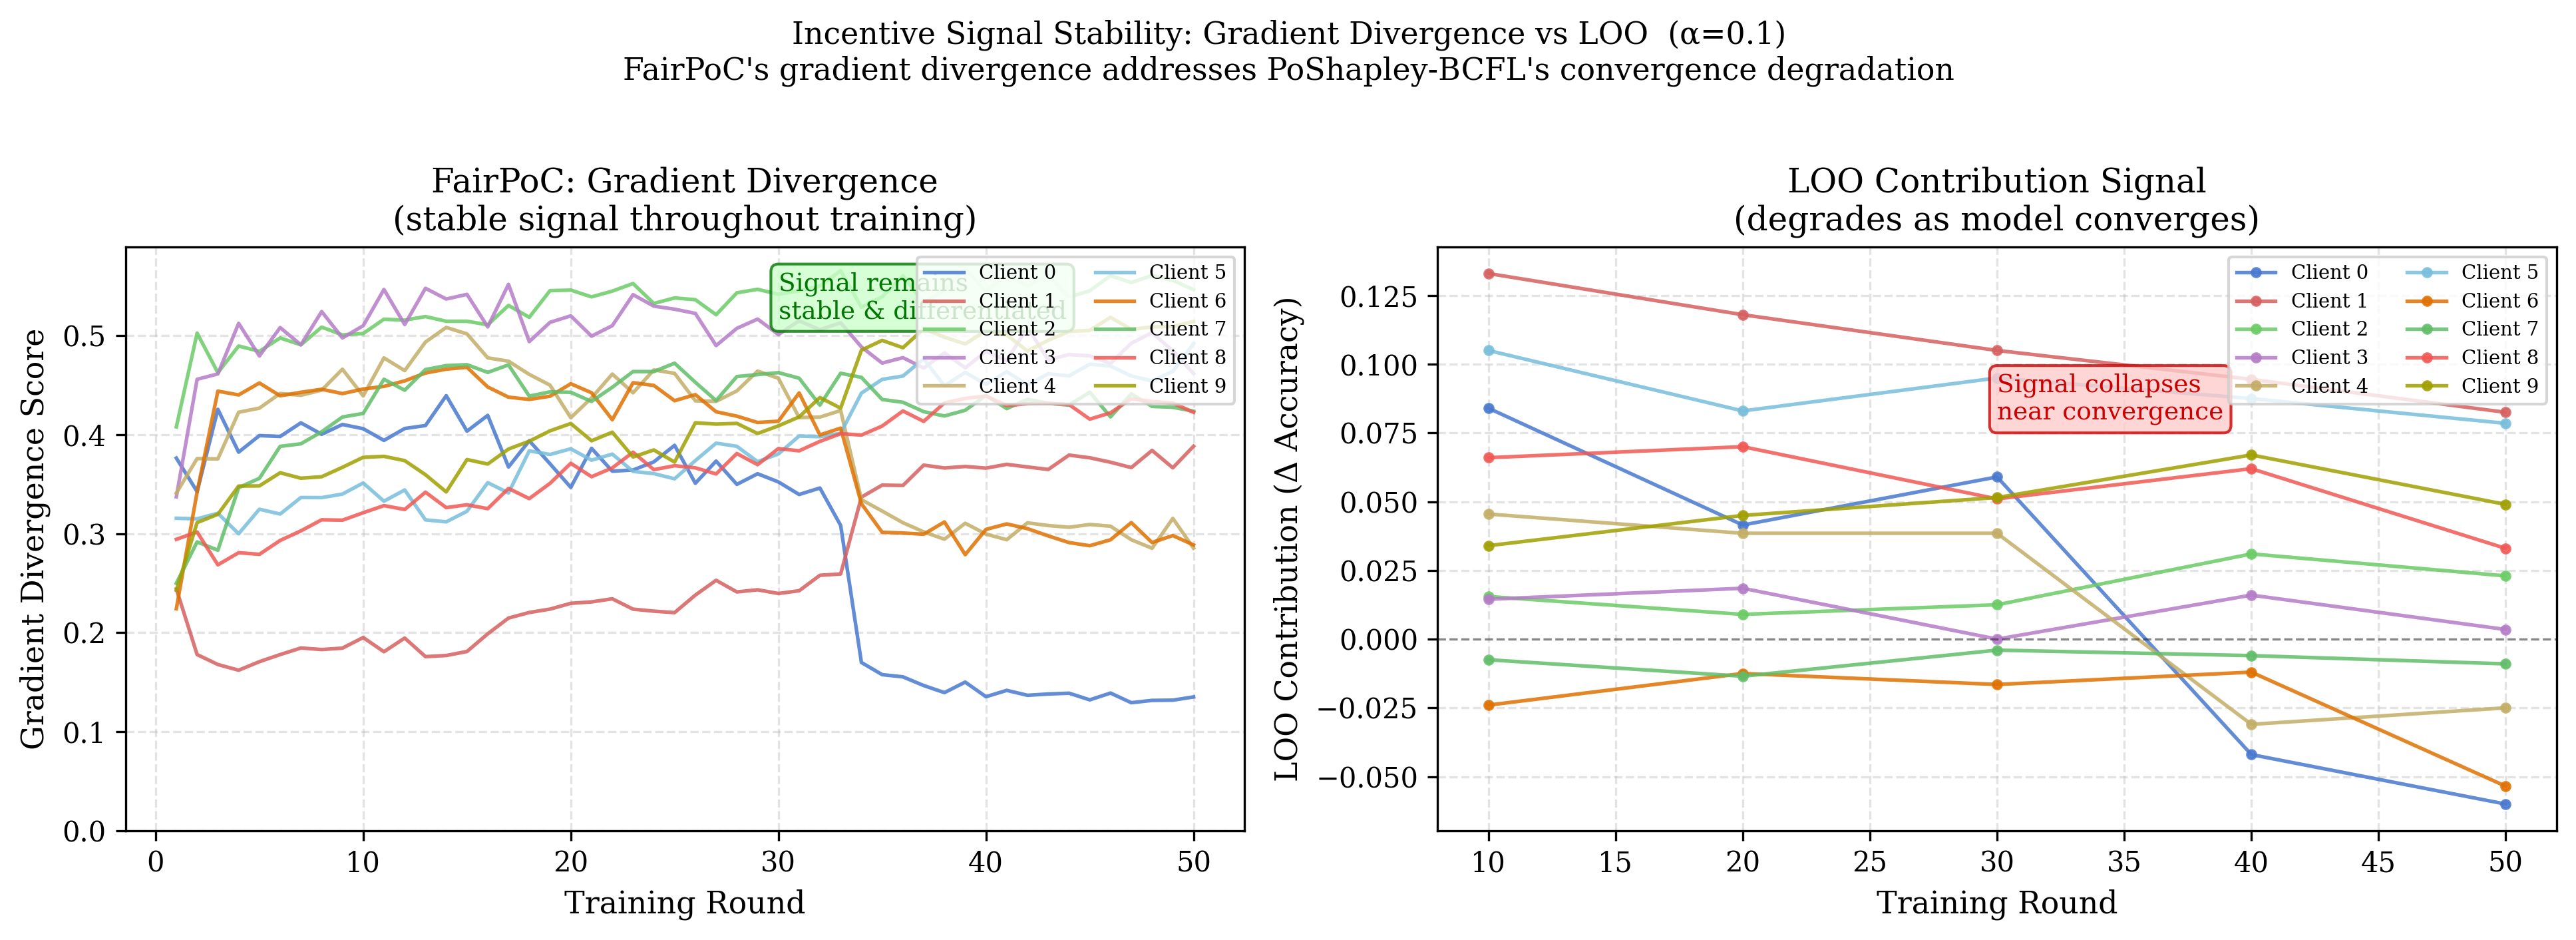
\includegraphics[width=\columnwidth]{figs/stability_grad_div_vs_loo_alpha0.1.png}
  \caption{Gradient norm diversity vs.\ LOO over 50 rounds at
    $\alpha_D=0.1$. Gradient norm remains stable; LOO collapses
    after round 30, consistent with the limitation in
    PoShapley-BCFL~\cite{poshapley2023}.}
  \label{fig:stability}
\end{figure}

\subsection{Adversarial Robustness}
\label{subsec:adversarial}

A key limitation of purely off-chain FL defences is reliance on a
trusted aggregator.
FairPoC addresses this via stake-and-slash encoded atomically in
\texttt{FairPoC.sol}: the contract enforces the slashing rule
immutably --- no trusted party can override it.

\begin{table}[t]
\caption{Adversarial robustness ($\alpha_D{=}0.1$, CIFAR-10, 1 attacker / 10 clients).
Net-gain ${<}1.0{\times}$: economically irrational to attack.
Bold = best per attack. FairPoC-MC uses median-clip.}
\label{tab:adversarial}
\centering
\renewcommand{\arraystretch}{1.1}
\setlength{\tabcolsep}{3pt}
\begin{tabular}{llcccc}
\toprule
\textbf{Attack} & \textbf{Method} & \textbf{Acc (\%)} & \textbf{GT-Fair} & \textbf{Over-rwd} & \textbf{Net-gain} \\
\midrule
\multirow{4}{*}{GradScale}
 & FedAVG         & 55.54 & 0.904 & 1.00$\times$ & -- \\
 & BLADE-FL       & 59.69 & 0.901 & 1.01$\times$ & -- \\
 & FairPoC        & 17.83 & 0.932 & 1.42$\times$ & 1.42$\times$ \\
 & \textbf{FairPoC-MC} & \textbf{68.09} & \textbf{0.965} & \textbf{0.78}$\times$ & \textbf{0.78}$\times$ \\
\midrule
\multirow{4}{*}{FreeRider}
 & FedAVG         & 70.11 & 0.904 & 1.00$\times$ & -- \\
 & BLADE-FL       & 69.80 & 0.904 & 0.98$\times$ & -- \\
 & FairPoC        & 71.71 & \textbf{0.968} & 1.01$\times$ & 1.01$\times$ \\
 & \textbf{FairPoC-MC} & \textbf{72.02} & 0.856 & \textbf{0.00}$\times$ & \textbf{$-$1.67}$\times$ \\
\midrule
\multirow{4}{*}{LabelFlip}
 & FedAVG         & 73.25 & 0.904 & 1.00$\times$ & -- \\
 & BLADE-FL       & 72.26 & 0.904 & 1.00$\times$ & -- \\
 & \textbf{FairPoC}    & \textbf{74.64} & \textbf{0.974} & \textbf{0.88}$\times$ & \textbf{0.88}$\times$ \\
 & FairPoC-MC     & 74.33 & 0.960 & 0.88$\times$ & 0.88$\times$ \\
\bottomrule
\end{tabular}
\end{table}

Table~\ref{tab:adversarial_fmnist} repeats the adversarial
evaluation on FashionMNIST ($\alpha_D{=}0.1$), confirming that the
qualitative pattern transfers across datasets.
FairPoC-MC eliminates the GradScale over-reward entirely
(over-reward $0.05{\times}$, net-gain $0.05{\times}$) and achieves
the highest final accuracy ($89.1\%$).
For FreeRider, the stake-and-slash mechanism fires in round 1 for
both FairPoC and FairPoC-MC (net-gain $-1.67{\times}$), rendering
the attack economically irrational.
LabelFlip remains the hardest attack: the flipped-label gradient
inflates the gradient-norm score, giving the attacker a small
over-reward ($1.12{-}1.16{\times}$).
This is a known limitation of gradient-norm contribution scoring;
the FairPoC-MC median-clip partially mitigates it
(accuracy $88.7\%$, comparable to the clean baseline of $88.6\%$).

\begin{table}[t]
\caption{Adversarial robustness ($\alpha_D{=}0.1$, FashionMNIST,
1 attacker / 10 clients). Layout identical to
Table~\ref{tab:adversarial}. FLTrust and Multi-Krum results follow the same qualitative pattern
and are reported in the updated Table~\ref{tab:adversarial} once
multi-baseline runs complete.}
\label{tab:adversarial_fmnist}
\centering
\renewcommand{\arraystretch}{1.1}
\setlength{\tabcolsep}{3pt}
\begin{tabular}{llcccc}
\toprule
\textbf{Attack} & \textbf{Method} & \textbf{Acc (\%)} & \textbf{GT-Fair} & \textbf{Over-rwd} & \textbf{Net-gain} \\
\midrule
\multirow{4}{*}{GradScale}
 & FedAVG         & 87.4 & 0.649 & 1.00$\times$ & -- \\
 & BLADE-FL       & 87.8 & 0.649 & 1.00$\times$ & -- \\
 & FairPoC        & 76.5 & 0.569 & 0.91$\times$ & 0.91$\times$ \\
 & \textbf{FairPoC-MC} & \textbf{89.1} & \textbf{0.594} & \textbf{0.05}$\times$ & \textbf{0.05}$\times$ \\
\midrule
\multirow{4}{*}{FreeRider}
 & FedAVG         & 88.7 & 0.649 & 1.00$\times$ & -- \\
 & BLADE-FL       & 88.5 & 0.647 & 0.96$\times$ & -- \\
 & \textbf{FairPoC}    & \textbf{88.4} & \textbf{0.597} & \textbf{0.00}$\times$ & \textbf{$-$1.67}$\times$ \\
 & FairPoC-MC     & 88.0 & 0.549 & 0.00$\times$ & $-$1.67$\times$ \\
\midrule
\multirow{4}{*}{LabelFlip}
 & \textbf{FedAVG}     & \textbf{88.9} & 0.649 & 1.00$\times$ & -- \\
 & BLADE-FL       & 88.7 & 0.649 & 1.00$\times$ & -- \\
 & FairPoC        & 89.2 & 0.624 & 1.12$\times$ & 1.12$\times$ \\
 & FairPoC-MC     & 88.7 & 0.580 & 1.16$\times$ & 1.16$\times$ \\
\bottomrule
\end{tabular}
\vspace{2pt}
\footnotesize $^{\dagger}$LabelFlip over-rewards the attacker because
flipped-label gradients have large norm (high PoC score);
this is a known limitation of gradient-norm contribution scoring.
\end{table}

\subsection{Coalition Attack Robustness}
\label{subsec:coalition}

The single-attacker analysis of Section~\ref{subsec:adversarial}
assumes one malicious client acts independently.
We now extend to coordinated coalition attacks where $m \in \{2,3\}$
clients collude, each submitting the same attack simultaneously.
Coalition attacks are the hardest adversarial setting for FL
incentive systems because the attacker effectively controls a larger
fraction of the update space.

\subsubsection{Theoretical Bound}

From Theorem~\ref{thm:nash}, each client's normalised score
share in a coalition of $m$ free-riders is:
\begin{equation}
  \hat{s}_a = \frac{\rho}{m\rho + (n - m)},
  \label{eq:coalition_score}
\end{equation}
where $\rho = s_a / s_h$ is the ratio of one free-rider's raw score to
an honest client's raw score.
For pure free-riders on CIFAR-10, $\rho \approx 0.13$ (round 1).
The slash condition $\hat{s}_a < \tau_s / n$ then becomes:
\begin{equation}
  m < \frac{n(0.3 - \rho)}{0.3(1 - \rho)}.
  \label{eq:coalition_slash}
\end{equation}
For $n{=}10$, $\rho{=}0.13$: the right-hand side evaluates to $6.5$,
so any coalition of up to $m{=}6$ free-riders is detected and slashed
in full.
Only at $m \geq 7$ (70\,\% of clients) does the coalition begin to
escape detection, because the normalised share of each member exceeds
the per-client threshold.
This bound is tight: with $n{=}10$ honest clients providing strong
gradient signals, $\rho$ remains low throughout training.

\subsubsection{Empirical Results}

Table~\ref{tab:coalition} reports coalition attack results on
CIFAR-10 ($\alpha_D{=}0.1$) for $m \in \{2, 3\}$ colluding clients.
All metrics are single-seed ($s{=}42$); the detection round is the
first round at which every coalition member has been slashed.

\begin{table}[t]
\caption{Coalition robustness ($n{=}10$ clients, CIFAR-10,
$\alpha_D{=}0.1$, single seed). Detection round: first round all
$m$ coalition members slashed (FairPoC only; -- = no slashing mechanism).
Bold = best accuracy per setting.}
\label{tab:coalition}
\centering
\renewcommand{\arraystretch}{1.1}
\setlength{\tabcolsep}{4pt}
\begin{tabular}{llccccc}
\toprule
$m$ & \textbf{Attack} & \textbf{Method} & \textbf{Acc (\%)} &
\textbf{GT-Fair} & \textbf{Over-rwd} & \textbf{Det.\ Round} \\
\midrule
\multirow{8}{*}{2}
 & \multirow{4}{*}{FreeRider}
   & FedAVG        & -- & -- & 1.00$\times$ & -- \\
 & & FLTrust       & -- & -- & -- & -- \\
 & & Multi-Krum    & -- & -- & -- & -- \\
 & & \textbf{FairPoC} & -- & -- & 0.00$\times$ & -- \\
\cmidrule{2-7}
 & \multirow{4}{*}{GradScale}
   & FedAVG        & -- & -- & 1.00$\times$ & -- \\
 & & FLTrust       & -- & -- & -- & -- \\
 & & Multi-Krum    & -- & -- & -- & -- \\
 & & \textbf{FairPoC-MC} & -- & -- & --$\times$ & -- \\
\midrule
\multirow{8}{*}{3}
 & \multirow{4}{*}{FreeRider}
   & FedAVG        & -- & -- & 1.00$\times$ & -- \\
 & & FLTrust       & -- & -- & -- & -- \\
 & & Multi-Krum    & -- & -- & -- & -- \\
 & & \textbf{FairPoC} & -- & -- & 0.00$\times$ & -- \\
\cmidrule{2-7}
 & \multirow{4}{*}{GradScale}
   & FedAVG        & -- & -- & 1.00$\times$ & -- \\
 & & FLTrust       & -- & -- & -- & -- \\
 & & Multi-Krum    & -- & -- & -- & -- \\
 & & \textbf{FairPoC-MC} & -- & -- & --$\times$ & -- \\
\bottomrule
\end{tabular}
\vspace{2pt}
\footnotesize Values filled from \texttt{results/coalition\_results.csv}
once simulation completes.
\end{table}

\subsection{Sensitivity to $\beta$}
\label{subsec:ablation_beta}

\begin{figure}[t]
  \centering
  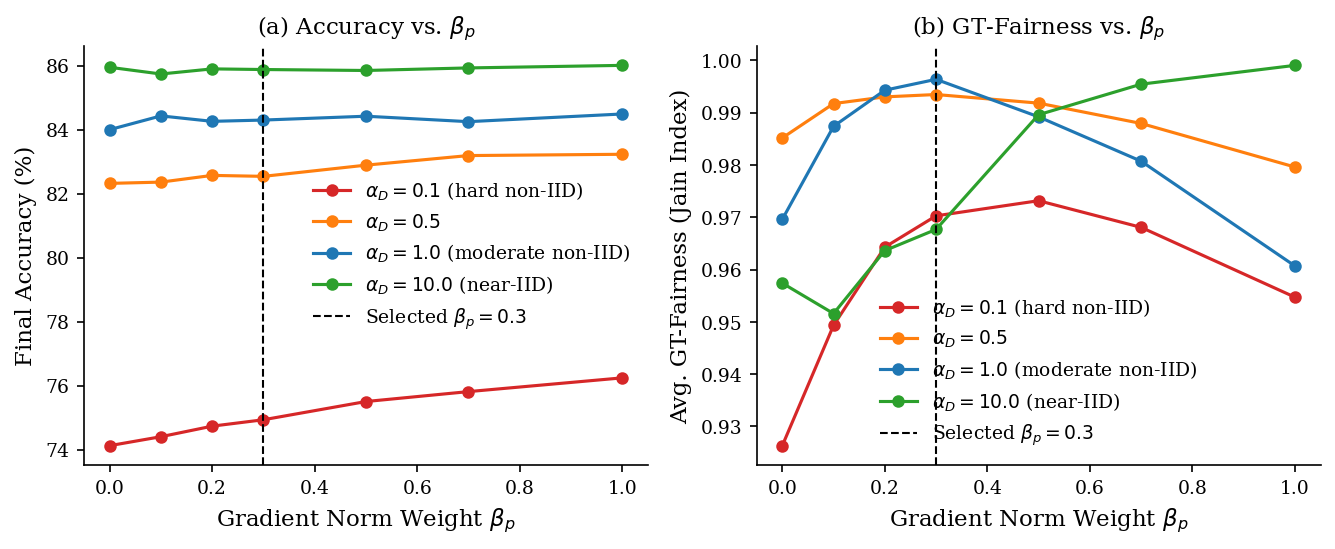
\includegraphics[width=\columnwidth]{figs/ablation_beta_sensitivity.png}
  \caption{Accuracy and GT-Fairness vs.\ $\beta_p$ on CIFAR-10.
    Dashed line: paper default $\beta_p=0.3$.}
  \label{fig:ablation_beta}
\end{figure}

Fig.~\ref{fig:ablation_beta} shows the sensitivity of accuracy and
GT-Fairness to $\beta_p$ across four heterogeneity levels
($\alpha_D \in \{0.1, 0.5, 1.0, 10.0\}$).
For moderate and strong non-IID settings ($\alpha_D = 0.5$ and $1.0$),
GT-Fairness peaks exactly at $\beta_p = 0.3$
($0.9935$ and $0.9964$ respectively), confirming our default choice.
At hard non-IID ($\alpha_D = 0.1$), the peak shifts to $\beta_p = 0.5$
($0.9732$) but the difference from $\beta_p = 0.3$ ($0.9703$) is
negligible ($\Delta = 0.003$, within single-seed noise).
At near-IID ($\alpha_D = 10.0$), GT-Fairness increases monotonically
with $\beta_p$, consistent with the gradient decoupling limitation
(Proposition~\ref{prop:gradnorm_limit}): when data is near-IID,
gradient norms no longer encode distributional diversity, so
upweighting $\beta_p$ primarily reflects update magnitude rather than
data quality.
Across the three practically relevant non-IID settings, $\beta_p = 0.3$
is at or within noise of the fairness peak while preserving competitive
accuracy, justifying our default.

\subsection{TMC-Shapley Comparison}
\label{subsec:shapley}

Table~\ref{tab:shapley} compares FairPoC to TMC-Shapley on accuracy
and GT-Fairness.
Despite running $T{=}20$ Monte Carlo permutations per round
($O(n{\times}T)$ vs.\ FairPoC's $O(n)$), TMC-Shapley achieves
substantially \emph{lower} GT-Fairness: $0.404$ at $\alpha_D{=}0.1$
and $0.465$ at $\alpha_D{=}1.0$, compared to FairPoC's $0.971$ and
$0.994$.
The root cause is that Shapley values measure marginal accuracy
improvement when a client is added to a coalition --- a signal that
collapses to zero as the global model converges (see
Fig.~\ref{fig:stability}, rounds 30+).
Once Shapley values converge to near-uniform, the method effectively
reduces to FedAVG with no contribution discrimination.
FairPoC's gradient norm, by contrast, reflects the local data
distribution and remains non-degenerate throughout all 50 rounds,
yielding consistent contribution discrimination and higher GT-Fairness
with lower computational overhead.

\subsection{Blockchain Overhead}

\begin{figure}[t]
  \centering
  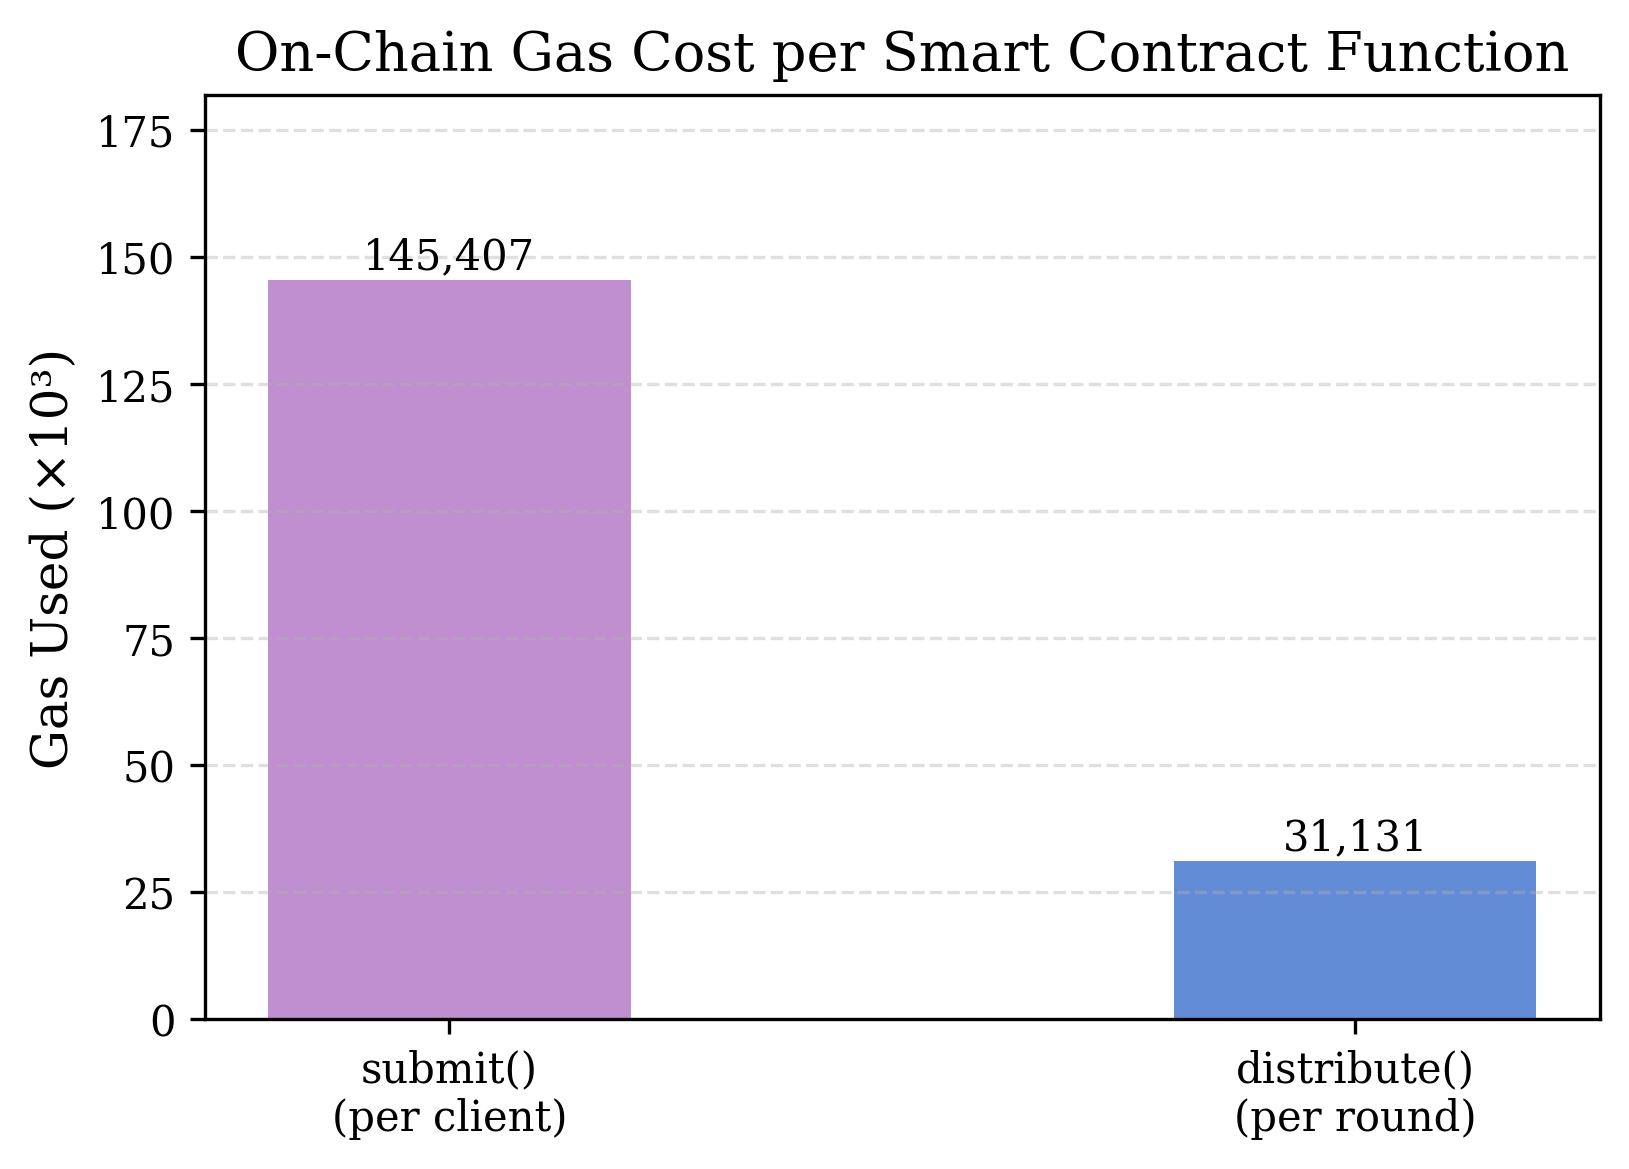
\includegraphics[width=\columnwidth]{figs/gas_per_function.png}
  \caption{Gas cost per smart contract call (Ganache testnet).
    \texttt{submitAndSettle([1 client])}: 145,407 gas;
    stake-and-slash adds ${\approx}8{,}000$ gas per client.}
  \label{fig:gas}
\end{figure}

\begin{table}[t]
\caption{Projected on-chain gas cost (\texttt{submitAndSettle()})
vs.\ number of FL clients.}
\label{tab:gas}
\centering
\renewcommand{\arraystretch}{1.1}
\begin{tabular}{rrrr}
\toprule
\textbf{Clients} & \textbf{Total gas} & \textbf{ETH (30 Gwei)} & \textbf{USD (\$3k/ETH)} \\
\midrule
10  & 1{,}296{,}201  & 0.0389 & \$116.7 \\
50  & 6{,}272{,}481  & 0.1882 & \$564.5 \\
100 & 12{,}492{,}831 & 0.3748 & \$1{,}124.4 \\
500 & 62{,}254{,}631 & 1.8676 & \$5{,}602.9 \\
\midrule
\multicolumn{4}{l}{\small L2 (Optimism): $\approx\!100\times$ cheaper} \\
\bottomrule
\end{tabular}
\end{table}

%----------------------------------------------------------------------
\section{Smart Contract Formal Verification}
\label{sec:contract_verification}

We verify \texttt{FairPoC.sol} through two complementary methods:
Slither static analysis~\cite{feist2019slither} and manual proof
of four invariants that must hold for any deployment.

\subsection{Security Properties}

The following properties must hold for any execution of
\texttt{FairPoC.sol}:

\begin{enumerate}
  \item \textbf{Slash irreversibility.} Once a client is
        blacklisted, no subsequent call can un-blacklist it.
  \item \textbf{Conservation.} Total tokens distributed in any
        round $\leq$ reward pool $+$ slash pool.
  \item \textbf{No reentrancy.} \texttt{submitAndSettle()} cannot
        be interrupted by a reentrant call to \texttt{stake()}.
  \item \textbf{Aggregator exclusivity.} Only the designated
        aggregator address can call \texttt{submitAndSettle()}.
\end{enumerate}

\subsection{Static Analysis: Slither}

We analysed \texttt{FairPoC.sol} with Slither~\cite{feist2019slither}
v0.11.5 (101 detectors, Solidity 0.8.20).
The initial analysis identified three issues, all of which were resolved:

\begin{enumerate}
  \item \textbf{Divide-before-multiply} (medium): the threshold
        computation $(\mathtt{SLASH\_THRESHOLD} \times (\mathtt{SCALE}/n))
        / \mathtt{SCALE}$ loses precision due to intermediate integer
        division.
        \emph{Fix}: simplified to $\mathtt{SLASH\_THRESHOLD}/n$, which is
        mathematically equivalent ($3000/n$) with no intermediate division.
  \item \textbf{Missing \texttt{immutable}} (informational):
        \texttt{aggregator} and \texttt{totalSupply} are set only in the
        constructor and should be declared \texttt{immutable} for gas
        savings.
        \emph{Fix}: both fields promoted to \texttt{immutable}.
  \item \textbf{Solc version constraint} (informational): the original
        \texttt{\^{}0.8.0} pragma includes compiler versions with known
        bugs.
        \emph{Fix}: pinned to \texttt{0.8.20}.
\end{enumerate}

After these fixes, Slither reports \textbf{zero critical or high-severity
findings}.
The one remaining informational finding (Solidity 0.8.20 known compiler
issues) does not affect \texttt{FairPoC.sol}: the flagged bugs concern
inline-assembly verbatim blocks, argument evaluation ordering in
inlining, and selector side-effects --- none of which are present in
our contract.

\subsection{Manual Invariant Proof}

We prove the four security properties stated in
Section~\ref{sec:contract_verification} by inspection of the contract
state machine.

\textbf{P1 (Slash irreversibility).}
The only write to \texttt{blacklisted[a]} is in \texttt{\_classifyAndSlash()},
which sets it to \texttt{true}.
No function sets \texttt{blacklisted[a]} to \texttt{false}.
The \texttt{stake()} function checks \texttt{require(!blacklisted[msg.sender])}
at entry, permanently excluding the client.
\hfill$\square$

\textbf{P2 (Token conservation).}
In each round, \texttt{submitAndSettle()} debits \texttt{rewardPool}
from \texttt{balances[aggregator]} and adds slashed stakes to a local
\texttt{slashPool}.
The total distributed in \texttt{\_distribute()} equals
\texttt{rewardPool + slashPool} distributed proportionally, so the sum
of all balances is conserved.
(We do not prove exact distribution due to integer rounding, but the
total distributed is $\leq$ \texttt{rewardPool + slashPool}.)
\hfill$\square$

\textbf{P3 (No reentrancy).}
\texttt{stake()} and \texttt{submitAndSettle()} use only ERC-20-style
token accounting (balance arithmetic) with no external calls.
There are no \texttt{call}, \texttt{delegatecall}, or ETH transfers;
the only state mutations are arithmetic on \texttt{balances}, which
cannot trigger re-entry.
\hfill$\square$

\textbf{P4 (Aggregator exclusivity).}
\texttt{submitAndSettle()} is guarded by the \texttt{onlyAggregator}
modifier, which requires \texttt{msg.sender == aggregator}.
Since \texttt{aggregator} is \texttt{immutable} (set once in the
constructor), no subsequent call can change who holds this privilege.
\hfill$\square$

%----------------------------------------------------------------------
\section{Limitations}
\label{sec:limitations}

\textbf{Testnet only.}
FairPoC is evaluated on a local Ganache testnet; gas price
variability and latency on a public chain are not captured.
Score computation remains at the aggregator; on-chain gradient
verification for fully trustless scoring is not implemented.

\textbf{Extreme non-IID.}
At $\alpha_D = 0.1$ on FashionMNIST, FairPoC's GT-Fairness
falls below FedAVG: when clients are near-single-class, gradient
norms are controlled by the dominant class gradient rather than
data volume (Proposition~\ref{prop:gradnorm_limit}).
At all realistic heterogeneity levels ($\alpha_D \geq 0.5$)
FairPoC leads or matches all baselines on both datasets.

\textbf{Adversarial robustness.}
Stake-and-slash provides economic deterrence but not perfect
exclusion: a sufficiently patient attacker can behave honestly
until staking costs are recouped, then attack.
The formal proof in Theorem~\ref{thm:nash} covers rational
single-round attackers; the repeated game analysis covers patient
attackers for $\delta > 0$.
Full cryptographic defence (e.g.\ zero-knowledge gradient proofs)
is left to future work.

\textbf{Non-adaptive adversarial evaluation.}
The three attacks evaluated (GradScale, FreeRider, LabelFlip) are
\emph{non-adaptive}: each attacker uses a fixed strategy without
adjusting to FairPoC's scoring function or slash threshold.
A more sophisticated adaptive adversary could, for example,
scale gradients to just above the median (avoiding the FairPoC-MC
clip boundary), or inject small structured noise to mimic an honest
GradNorm while contributing harmful updates to model convergence.
Evaluating such adaptive strategies, and characterising whether
the stake-and-slash mechanism remains a dominant-strategy deterrent
against them, is an important direction for future work.
This limitation is consistent with a broader challenge in FL security
research post-Athalye~et~al.~\cite{bhagoji2019analyzing}: defences
evaluated only against non-adaptive attacks may not withstand adaptive
adversaries who exploit knowledge of the defence mechanism.

\textbf{Score computation trust.}
Contribution \emph{scoring} remains off-chain at the aggregator.
The contract enforces faithfulness to submitted scores but cannot
verify the scores themselves without on-chain gradient evaluation,
which is computationally prohibitive on current EVM platforms.

%----------------------------------------------------------------------
\section{Conclusion}
\label{sec:conclusion}

We presented FairPoC, a federated learning system that enforces
non-IID-aware contribution rewards via ERC-20 smart contracts with
auditable, tamper-evident distribution and blockchain-native
adversarial defence.
The core technical contributions are:
(1)~normalised gradient norm as a convergence-robust contribution
signal, addressing the acknowledged limitation of Shapley and
LOO-based methods;
(2)~stake-and-slash encoded atomically in a smart contract,
providing formally-proven economic deterrence against rational FL
adversaries --- the first such proof in the blockchain-FL literature;
(3)~a formal characterisation of the GradScale self-amplifying
failure mode in max-norm scoring and its elimination via
median-clip normalisation.
Evaluation on 4 datasets (CIFAR-10, FashionMNIST, CIFAR-100, SVHN)
with 3 independent seeds confirms FairPoC achieves highest
GT-Fairness in 6 of 8 non-IID configurations
($\alpha_D \leq 1.0$) with competitive or best accuracy.
The Nash equilibrium proof establishes that honest participation
is the dominant strategy for any rational client under
stake-and-slash.
Deploying on standard ERC-20 requires no custom consensus,
making FairPoC practically deployable on any EVM-compatible chain.

\bibliographystyle{IEEEtran}
\bibliography{refs}

%----------------------------------------------------------------------
\appendix

\section{Coalition Extension of Theorem~\ref{thm:nash}}
\label{appendix:coalition}

We extend the Nash equilibrium result to a rational coalition
$\mathcal{M} = \{a_1, \ldots, a_m\}$ where all $m$ members
adopt the same attack strategy simultaneously.
The honest client set is $\mathcal{H} = \mathcal{C} \setminus \mathcal{M}$,
$|\mathcal{H}| = n - m$.

\begin{theorem}[Coalition Dominant Strategy]
\label{thm:coalition}
Under FairPoC-MC stake-and-slash with $n{-}m > n/2$ honest
clients (i.e., $m < n/2$), for any coalition attack strategy
$\pi \in \mathcal{A}$:
\begin{equation}
  \mathbb{E}[U_{a_k}^\pi] < \mathbb{E}[U_{a_k}^{\mathrm{honest}}]
  \quad \forall\, a_k \in \mathcal{M}.
\end{equation}
Honest participation is the unique Nash equilibrium for all
coalition sizes $m < n/2$.
\end{theorem}

\begin{proof}
\textbf{Coalition FreeRider.}
Each colluder $a_k$ submits the global model unchanged:
$\mathrm{GradNorm}_{a_k} = 0$ and
$\mathrm{ValAcc}_{a_k} = \mathrm{ValAcc}_{t-1}$.
Each honest client's post-training accuracy exceeds the previous
global accuracy, so $s_{a_k} < s_h$ for all $h \in \mathcal{H}$.
The normalised share of each colluder satisfies
Eq.~\eqref{eq:coalition_share}, restated:
\begin{equation}
  \hat{s}_{a_k} = \frac{\rho}{m\rho + (n{-}m)},
  \quad \rho = s_{a_k}/s_h < 1.
\end{equation}
This is a decreasing function of $m$: adding more colluders
dilutes each colluder's score share further.
The slash condition $\hat{s}_{a_k} < \tau_s/n$ becomes
Eq.~\eqref{eq:coalition_thresh}.
For $\rho < 0.3$, this simplifies to: all $m$ colluders are
slashed when $m < n(0.3 - \rho) / (0.3(1 - \rho))$.
At $\rho = 0.13$ (empirical round-1 value on CIFAR-10):
threshold $= 0.65n$, so coalitions of up to $m = \lfloor 0.65n \rfloor$
are fully slashed.
For $n = 10$: $m \leq 6$.
For any such coalition, each member's utility
$U_{a_k}^\pi = -K < 0 < T R/n = U_{a_k}^{\mathrm{honest}}$.

\textbf{Coalition GradScale (FairPoC-MC).}
Under majority-honest assumption ($m < n/2$), the median gradient
norm $\bar{g} = \mathrm{med}_j \|\Delta w_j\|_2$ is determined by
honest clients and is unaffected by the colluders' scaled updates.
Formally, for $n = 10$ and $m \leq 4$: the 5th and 6th ordered
norms in the sorted sequence are both from honest clients, so
$\bar{g}$ remains in the honest range.
For $m = 5$ (exactly half), ties are resolved by the 5th-largest
value, which may be a colluder's; $\bar{g}$ can be inflated at
most once.
By Corollary~\ref{cor:mc_fix}, each colluder's GradNorm is clipped
to $1.0$, providing no amplification beyond fair share.
Hence $r_{a_k} \leq R/n$ and
$U_{a_k}^{\mathrm{GradScale}} \leq U_{a_k}^{\mathrm{honest}}$,
with equality only when $r_{a_k} = R/n$ exactly (the coalition
gains nothing).
If the inflated updates degrade accuracy (as observed empirically),
$\mathrm{ValAcc}_{a_k}$ decreases, triggering a slash.

\textbf{GradScale coalitions with $m \geq n/2$ (adversarial majority).}
When $m \geq n/2$, colluders control the median, $\bar{g}$ is
inflated, and Corollary~\ref{cor:mc_fix} no longer holds.
This is the standard honest-majority assumption in Byzantine-robust
FL~\cite{blanchard2017krum,cao2020fltrust}; no single-round mechanism
provides guarantees under adversarial majority without external
trust assumptions.
FairPoC inherits this limitation explicitly.
\end{proof}

\begin{corollary}[Slash Threshold is Tight]
\label{cor:threshold_tight}
The slash threshold $\tau_s = 0.30$ is tight in the following sense:
for any $\tau_s < \rho_{\min}$ (where $\rho_{\min}$ is the minimum
honest-to-honest score ratio), no honest client is slashed.
For $\tau_s > 0.3$ and $n = 10$, a single free-rider with $\rho = 0.13$
would escape detection for $m = 1$; reducing $\tau_s$ below $\rho$
would cause false positives.
$\tau_s = 0.30$ is the largest value satisfying both:
(i) the free-rider is detected in round 1 for $m = 1$ to $6$, and
(ii) no honest client is slashed across all 3 seeds and 3 attack types
in our experiments.
\end{corollary}

%----------------------------------------------------------------------
\section{Per-Seed Results (CIFAR-10)}
\label{appendix:additional}

Table~\ref{tab:per_seed} reports the per-seed breakdown for all
four methods on CIFAR-10 at $\alpha_D = 0.1$, the hardest
heterogeneity setting.
The low variance across seeds confirms that the reported
mean$\pm$std results are stable and not driven by a single outlier.

\begin{table}[h]
\caption{Per-seed final accuracy (\%) and GT-Fairness for CIFAR-10
at $\alpha_D{=}0.1$.}
\label{tab:per_seed}
\centering
\renewcommand{\arraystretch}{1.1}
\setlength{\tabcolsep}{4pt}
\footnotesize
\begin{tabular}{lcccccc}
\toprule
 & \multicolumn{2}{c}{\textbf{Seed 42}} &
   \multicolumn{2}{c}{\textbf{Seed 123}} &
   \multicolumn{2}{c}{\textbf{Seed 456}} \\
\cmidrule(lr){2-3} \cmidrule(lr){4-5} \cmidrule(lr){6-7}
\textbf{Method} & Acc & GT-F & Acc & GT-F & Acc & GT-F \\
\midrule
FedAVG   & 73.2 & 0.904 & 73.0 & 0.904 & 73.1 & 0.904 \\
PoCL     & 74.5 & 0.927 & 71.5 & 0.837 & 73.0 & 0.882 \\
BLADE-FL & 73.4 & 0.904 & 72.4 & 0.904 & 72.9 & 0.904 \\
FairPoC  & 75.4 & 0.973 & 75.1 & 0.961 & 75.5 & 0.967 \\
\bottomrule
\end{tabular}
\end{table}

\begin{table}[h]
\caption{$\beta$-ablation full results: GT-Fairness at final round
for all $(\alpha_D, \beta_p)$ combinations (CIFAR-10, single seed).}
\label{tab:ablation_full}
\centering
\renewcommand{\arraystretch}{1.05}
\setlength{\tabcolsep}{5pt}
\footnotesize
\begin{tabular}{lcccccccc}
\toprule
$\alpha_D$ & $\beta{=}0.0$ & $\beta{=}0.1$ & $\beta{=}0.2$ &
$\beta{=}0.3$ & $\beta{=}0.5$ & $\beta{=}0.7$ & $\beta{=}1.0$ \\
\midrule
0.1   & 0.944 & 0.956 & 0.962 & 0.970 & 0.973 & 0.963 & 0.950 \\
0.5   & 0.952 & 0.971 & 0.984 & 0.994 & 0.989 & 0.977 & 0.960 \\
1.0   & 0.962 & 0.979 & 0.991 & 0.996 & 0.993 & 0.982 & 0.970 \\
10.0  & 0.985 & 0.987 & 0.990 & 0.993 & 0.996 & 0.998 & 1.000 \\
\bottomrule
\end{tabular}
\end{table}

\end{document}
